\documentclass[a4paper,12pt]{article}
\usepackage[vietnamese]{babel}
\usepackage[utf8]{vietnam} % Có thể không cần nếu dùng fontspec
\usepackage{amsmath}
\usepackage{graphicx}
\usepackage{booktabs}
\usepackage[a4paper, margin=1in]{geometry}
\usepackage{microtype}
\usepackage{enumitem}
\usepackage{hyperref}
\usepackage{float}
\usepackage{array}
\usepackage{multirow}
\usepackage{tabularx}

\begin{document}

% Trang bìa
\begin{titlepage}
    \centering
    \vspace*{2cm}
    {\LARGE \textbf{BÁO CÁO PHÂN TÍCH BÀI BÁO}}\\[1.5cm]
    {\Large \textit{ChatGPT, Trí tuệ Nhân tạo Tạo sinh, Mô hình Ngôn ngữ Lớn và Tư vấn Đầu tư}}\\[1cm]
    \vspace{2cm}
    \textbf{Tác giả chính của bài báo:}\\[0.2cm]
    Lei Huang, Fangzhou Lu, Sixuan Li\\[1cm]
    \textbf{Người thực hiện báo cáo:}\\[0.2cm]
    Nguyễn Vũ Quang Anh\\
    Trịnh Tuấn Ngọc Bảo\\
    Phan Trần Mạnh Cường\\[1cm]
    \vspace{3cm}
    \textbf{Ngày thực hiện:} \today
    \vfill
\end{titlepage}

\tableofcontents
\newpage


% Abstract
\section*{\begin{center}
    \textbf{\LARGE Tóm tắt}
\end{center}
}
\noindent
Các mô hình ngôn ngữ lớn (LLMs), bao gồm cả ChatGPT, tận dụng khả năng suy luận của mình để tạo ra các đề xuất danh mục đầu tư vượt xa khả năng phân tích văn bản thông thường. Bằng cách tinh chỉnh mô hình LLM với dữ liệu huấn luyện cụ thể và điều chỉnh các tham số của ChatGPT để tăng cường tính linh hoạt đầu ra, có tiềm năng để ChatGPT tạo ra các danh mục đầu tư vượt trội so với các chuẩn mực thị trường trong các thử nghiệm ngoài mẫu.

\noindent
Sử dụng hai loại dữ liệu văn bản khác nhau bằng các ngôn ngữ khác nhau – các bài báo từ Wall Street Journal ở Hoa Kỳ và các thông báo chính sách từ chính phủ Trung Quốc – nhóm tác giả chỉ ra rằng ChatGPT có thể tạo ra các danh mục đầu tư với hệ số \textbf{alpha ba yếu tố hàng tháng lên tới 3\%}, đặc biệt là khi phản ứng với các tin tức liên quan đến chính sách. Khi so sánh kết quả này với những phương pháp phân tích văn bản truyền thống, nghiên cứu cho thấy phương pháp truyền thống không tạo ra được các danh mục đầu tư có alpha dương.

\newpage

% Introduction
\section{Giới thiệu}

\subsection{Bối cảnh}
Trong những năm gần đây, trí tuệ nhân tạo (AI) đã trở thành một trong những công nghệ chủ chốt định hình lại nhiều lĩnh vực, trong đó có tài chính. Đặc biệt, sự phát triển của các mô hình \textbf{Generative AI} như ChatGPT – một mô hình ngôn ngữ lớn (LLM) dựa trên kiến trúc Transformer – đã mở ra tiềm năng to lớn trong việc xử lý và khai thác dữ liệu văn bản khổng lồ trên Internet, báo chí, mạng xã hội,… để hỗ trợ ra quyết định đầu tư.

Tuy nhiên, trong lĩnh vực tài chính, việc ra quyết định đầu tư đòi hỏi không chỉ dựa trên dữ liệu định lượng truyền thống mà còn cần phân tích dữ liệu phi cấu trúc như tin tức, chính sách, tâm lý thị trường. Điều này đặt ra câu hỏi quan trọng: liệu một mô hình Generative AI như ChatGPT, vốn không được huấn luyện đặc biệt cho lĩnh vực tài chính, có thể cung cấp những gợi ý đầu tư hợp lý dựa trên dữ liệu văn bản không?

\subsection{Nội dung nghiên cứu}
Nghiên cứu của Lei Huang, Fangzhou Lu và Sixuan Li đã tìm hiểu về khả năng của ChatGPT trong việc trích xuất thông tin từ tin tức (WSJ, chính sách Trung Quốc) và gợi ý danh mục đầu tư. Bằng cách sử dụng ChatGPT với các tham số khác nhau (temperature, top-p), đồng thời so sánh với phân tích của chuyên gia tài chính, nhóm nghiên cứu kiểm tra:
\begin{itemize}
    \item ChatGPT có thể tạo ra các danh mục đầu tư hiệu quả cao hay không?
    \item Độ tin cậy của các gợi ý này khi áp dụng vào thực tế (in-sample và out-of-sample)?
    \item Sự khác biệt giữa ChatGPT 3.5 và ChatGPT 4.0, cùng tác động của fine-tuning trên dữ liệu tài chính.
\end{itemize}

\subsection{Mục tiêu nghiên cứu}
Nghiên cứu kiểm tra tiềm năng ứng dụng Generative AI trong gợi ý đầu tư, đồng thời đánh giá tính khả thi, ưu điểm, hạn chế của cách tiếp cận này. Nghiên cứu không chỉ mang ý nghĩa học thuật mà còn có thể gợi mở hướng đi mới cho xây dựng các hệ thống robo-advisor thông minh.

\subsection{Cơ sở lý thuyết và nghiên cứu liên quan}
\begin{itemize}
    \item \textbf{Generative AI và LLM:} GPT dựa trên kiến trúc Transformer, có khả năng học ngữ cảnh và sinh văn bản tự nhiên. ChatGPT là ứng dụng của LLM, được huấn luyện từ lượng lớn văn bản, có thể trả lời câu hỏi, tóm tắt và suy luận từ thông tin ngôn ngữ. Tham số ảnh hưởng: \textit{temperature}, \textit{top-p}, \textit{context window}.
    \item \textbf{Ra quyết định đầu tư và phân tích dữ liệu phi cấu trúc:} Dữ liệu lớn và phân tích cảm xúc thị trường (sentiment analysis) cho thấy tầm quan trọng của tin tức, chính sách, mạng xã hội.
    \item \textbf{Nghiên cứu liên quan:}
    \begin{itemize}
        \item Bollen et al. (2011): dự báo Dow Jones từ cảm xúc Twitter.
        \item Fung et al. (2020): phân tích tin tức Trung Quốc và tác động thị trường.
        \item Wu et al. (2022): đánh giá hiệu quả mô hình Transformer (BERT, GPT) trên văn bản tài chính.
    \end{itemize}
    \item \textbf{Khoảng trống nghiên cứu và đóng góp:} Ứng dụng trực tiếp ChatGPT để gợi ý đầu tư từ tin tức, chính sách vẫn còn mới mẻ. Nghiên cứu đóng góp bằng cách so sánh ChatGPT với chuyên gia, khảo sát tác động của tham số (temperature, top-p) và phiên bản (3.5 vs 4.0).
\end{itemize}

\subsection{Phương pháp nghiên cứu}

\subsubsection{Mục tiêu}
Mục tiêu của nghiên cứu này là kiểm định khả năng của mô hình ngôn ngữ lớn (LLMs), đặc biệt là ChatGPT, trong việc xử lý và phân tích dữ liệu văn bản tài chính không có cấu trúc, từ đó đưa ra khuyến nghị đầu tư một cách hợp lý và hiệu quả. Câu hỏi trung tâm là liệu ChatGPT có thể tạo ra các danh mục đầu tư có hiệu suất vượt trội so với các phương pháp phân tích văn bản truyền thống, xét theo chỉ tiêu lợi nhuận điều chỉnh theo rủi ro (alpha) trong mô hình Fama-French ba yếu tố và các mô hình mở rộng.



\subsubsection{Dữ liệu sử dụng}
Nghiên cứu sử dụng hai nguồn dữ liệu văn bản lớn và có tính đa dạng ngôn ngữ, bối cảnh:

\begin{itemize}
    \item \textbf{Tin tức tài chính từ Wall Street Journal (WSJ)} trong giai đoạn từ tháng 1 năm 2020 đến tháng 8 năm 2023. Đây là nguồn dữ liệu chính trong phân tích thị trường Hoa Kỳ.
    \item \textbf{Thông báo chính sách chính thức từ Quốc vụ viện Trung Quốc (State Council)} và các bộ ngành trực thuộc, với dữ liệu thu thập từ năm 2004 đến năm 2023. Đây là nguồn dữ liệu chính trong phân tích thị trường Trung Quốc.
\end{itemize}

\subsubsection{Phương pháp tiếp cận}
Quy trình phân tích được thiết kế mô phỏng theo cách một nhà đầu tư tương tác với cố vấn tài chính, bao gồm các bước:

\begin{enumerate}
    \item \textbf{Tiền xử lý dữ liệu}: Chuẩn hoá văn bản đầu vào, loại bỏ các yếu tố nhiễu, phân loại tin tức theo chủ đề bằng mô hình LDA (Latent Dirichlet Allocation), ví dụ như: chính trị, năng lượng, COVID-19,...
    
    \item \textbf{Tạo prompt cho ChatGPT}: Thiết kế câu lệnh truy vấn (prompt) dưới dạng hội thoại mô phỏng vai trò của một chuyên gia phân tích tài chính, yêu cầu ChatGPT đọc và đưa ra danh sách 5 cổ phiếu phù hợp cho từng bài báo hoặc thông cáo chính sách.

    \item \textbf{Điều chỉnh tham số đầu ra}: Sử dụng các tham số chính như \textit{temperature} (kiểm soát mức độ sáng tạo và ngẫu nhiên) và \textit{top-p} (nội suy theo xác suất) để đa dạng hóa phản hồi, từ đó mô phỏng các khuyến nghị từ nhiều chuyên gia tài chính khác nhau.

    \item \textbf{So sánh với phương pháp truyền thống}: Áp dụng phương pháp phân tích văn bản kinh điển (như đo độ tương đồng cosine giữa nội dung tin tức và báo cáo tài chính/earning calls của công ty) để chọn ra cổ phiếu liên quan, làm cơ sở đối chiếu với kết quả của ChatGPT.
\end{enumerate}

\subsubsection{Đánh giá hiệu suất}
Hiệu suất các danh mục được đánh giá bằng cách xây dựng danh mục đầu tư dựa trên khuyến nghị từ ChatGPT, sau đó đo lường lợi nhuận điều chỉnh rủi ro theo các mô hình định giá tài sản:

\begin{itemize}
    \item Mô hình Fama-French 3 yếu tố (FF3): bao gồm yếu tố thị trường, quy mô và giá trị.
    \item Mô hình 5 yếu tố (FF5): bổ sung khả năng sinh lợi và đầu tư.
    \item Mô hình mở rộng (FF5 + MOM + REV): thêm yếu tố đà tăng (momentum) và đảo chiều ngắn hạn (reversal).
\end{itemize}

Hệ số alpha được sử dụng như một chỉ tiêu đánh giá chính. Nếu alpha dương và có ý nghĩa thống kê, danh mục được xem là tạo ra lợi nhuận vượt trội so với thị trường sau khi đã điều chỉnh các yếu tố rủi ro.

\subsubsection{Kiểm tra độ tin cậy}
Kiểm tra tính hợp lý: Nhờ chuyên gia và sinh viên tài chính đánh giá xem các gợi ý của ChatGPT có hợp lí hay không.
\\ Kiểm tra khả năng dự báo bằng cách chia thành 2 giai đoạn

\begin{itemize}
    \item \textbf{In-sample}: Giai đoạn từ tháng 1/2020 đến 9/2021 (với dữ liệu WSJ) – thời kỳ dữ liệu nằm trong tập huấn luyện của ChatGPT.
    \item \textbf{Out-of-sample}: Giai đoạn từ tháng 10/2021 đến 9/2023 – ChatGPT chưa được tiếp cận trong quá trình huấn luyện, do đó cho phép kiểm định khả năng dự báo thực sự.
\end{itemize}

Cách chia giai đoạn tương tự được áp dụng cho dữ liệu Trung Quốc (2004–2021 là in-sample, 2021–2023 là out-of-sample).
\\ Thử nghiệm với các danh mục có thời gian nắm giữ từ 1 ngày đến 1 năm


\subsubsection{So sánh giữa các phiên bản ChatGPT}
Nghiên cứu tiến hành đối chiếu giữa các phiên bản khác nhau của mô hình:

\begin{itemize}
    \item \textbf{ChatGPT 3.5}: Phiên bản phổ biến, ổn định và có hiệu suất tốt trong việc đưa ra khuyến nghị logic.
    \item \textbf{ChatGPT 4.0}: Phiên bản nâng cao, tuy nhiên kết quả cho thấy đôi khi hiệu suất không vượt trội so với 3.5.
    \item \textbf{Fine-tuning (Tùy chỉnh mô hình)}: ChatGPT được tinh chỉnh bằng dữ liệu tài chính chuyên biệt (ví dụ: chọn cổ phiếu có hiệu suất cao nhất trong cùng ngành – cùng mã SIC – với khuyến nghị gốc của ChatGPT), giúp nâng cao độ chính xác và khả năng dự đoán của mô hình.
\end{itemize}

Việc tinh chỉnh giúp cải thiện đáng kể hiệu suất alpha out-of-sample, đặc biệt trong các nhóm tin tức chính sách và chính trị.


\subsection{Kết quả chính}

Nghiên cứu cho thấy ChatGPT có khả năng đưa ra các khuyến nghị đầu tư hợp lý và có hiệu quả dự báo nhất định. Cụ thể:

\begin{itemize}
    \item \textbf{Tính hợp lý của khuyến nghị:} Trong quá trình đánh giá bằng tay, khoảng 85–90\% khuyến nghị của ChatGPT được các chuyên gia tài chính và sinh viên chuyên ngành đánh giá là hợp lý. Điều này cho thấy mô hình có khả năng hiểu và xử lý văn bản chính sách, tin tức tài chính theo cách phù hợp với lập luận của con người.
    
    \item \textbf{Hiệu suất đầu tư in-sample:} Trong giai đoạn in-sample, danh mục đầu tư do ChatGPT đề xuất có hệ số alpha ba yếu tố (Fama-French) hàng ngày đạt tới 14.1 basis points (bps) khi tham số nhiệt độ được đặt là 1, tương đương khoảng 2.6\% lợi nhuận mỗi tháng. Điều này cho thấy tiềm năng của mô hình trong việc nhận diện thông tin giá trị từ dữ liệu đã học.

    \item \textbf{Hiệu suất out-of-sample:} Dù hiệu suất có giảm, ChatGPT vẫn tạo ra danh mục có alpha dương và có ý nghĩa thống kê trong giai đoạn out-of-sample – đặc biệt với các tin tức chính trị, với alpha hàng ngày lên tới 7 bps (tương đương khoảng 1.4\% mỗi tháng).

    \item \textbf{Tác động của fine-tuning:} Khi tinh chỉnh mô hình trên dữ liệu tài chính đặc thù, hiệu suất alpha tăng mạnh – lên tới 3\% mỗi tháng cho các danh mục dựa trên tin tức chính trị hoặc chính sách Trung Quốc. Mô hình sau khi tinh chỉnh được đánh giá có khuyến nghị hợp lý trong hơn 93\% trường hợp.

    \item \textbf{Khả năng vượt trội so với phân tích văn bản truyền thống:} Các phương pháp truyền thống (ví dụ: cosine similarity giữa nội dung tin tức và báo cáo tài chính) không tạo ra danh mục có alpha dương, cho thấy ChatGPT vượt trội trong việc trích xuất và suy luận từ thông tin phi cấu trúc.
\end{itemize}

\subsection{Kết luận}

Từ các kết quả thu được, nghiên cứu kết luận rằng ChatGPT – một mô hình Generative AI không được huấn luyện chuyên biệt cho tài chính – vẫn có khả năng hoạt động như một công cụ tư vấn đầu tư hiệu quả. Nhờ khả năng suy luận từ văn bản phức tạp và không cần cấu trúc cụ thể, ChatGPT có thể:

\begin{itemize}
    \item Gợi ý cổ phiếu phù hợp với tin tức chính sách hoặc kinh tế,
    \item Thích ứng với các bối cảnh ngôn ngữ khác nhau (tiếng Anh, tiếng Trung),
    \item Tạo ra danh mục đầu tư có khả năng sinh lời vượt trội.
\end{itemize}
Nghiên cứu mở ra hướng ứng dụng tiềm năng cho việc phát triển các hệ thống robo-advisor dựa trên mô hình ngôn ngữ lớn. Đồng thời, kết quả cũng góp phần khẳng định vai trò ngày càng quan trọng của AI trong lĩnh vực tài chính định lượng, đặc biệt trong bối cảnh thị trường chịu ảnh hưởng ngày càng mạnh từ các thông tin chính sách và phi cấu trúc.

\section{Chi tiết tổ chức}
\subsection{Trí tuệ nhân tạo Tạo sinh và ChatGPT}
ChatGPT, viết tắt của Chatbot Generative Pre-trained Transformer, là một mô hình ngôn ngữ tiên tiến và tinh vi được phát triển bởi OpenAI. Là một ví dụ đại diện cho AI tạo sinh, nó đã được huấn luyện trên một lượng lớn dữ liệu văn bản đa dạng để hiểu các mẫu ngôn ngữ phức tạp và tạo ra các phản hồi liên quan đến ngữ cảnh trong một buổi trò chuyện. Thông qua việc sử dụng kiến trúc transformer và các kỹ thuật học máy tiên tiến, ChatGPT có thể xử lý và hiểu ngôn ngữ của con người một cách hiệu quả, giúp nó có khả năng tham gia vào các cuộc trò chuyện mạch lạc và phù hợp với ngữ cảnh.
\\ Chat GPT thể hiện một loạt các chức năng, như viết sáng tạo, tạo nội dung và dịch ngôn ngữ. Đặc biệt, khả năng lý luận của nó nổi bật như một khía cạnh quan trọng và khác biệt, bao gồm tư duy logic, suy luận các mối liên hệ giữa các khía niệm khác nhau, và rút ra các kết luận thông minh.
\\ ChatGPT đã được trải qua việc đánh giá nghiêm ngặt nhằm kiểm tra khả năng lý luận của nó, bao gồm vượt qua accs bài kiểm tra tiêu chuẩn hoá như LSAT (Bài kiểm tra đầu vào trường luật), SAT (Bài kiểm tra đánh giá học thuật), GRE(Bài kiểm tra Hồ sơ sau đại học), ...
\\ Với việc vượt qua các bài test trên, chứng minh được ChatGPT thực sự có khả năng lý luận ấn tượng, như tư duy phản biện, hiểu đọc, phân tích dữ liệu và ra quyết định. Chứng cứ mạnh mẽ này càng củng cố lý do sử dụng ChatGPT để phân tích tin tức và thông báo chính trị cũng như đưa ra khuyến nghị đầu tư trong bài nghiên cứu này.

\subsection{ChatGPT Fine-Tuning}

\noindent
\textbf{Định nghĩa:}  
Fine-tuning là quá trình huấn luyện lại một mô hình ngôn ngữ lớn đã được huấn luyện trước, ví dụ như ChatGPT, trên một tập dữ liệu chuyên biệt nhằm điều chỉnh mô hình cho phù hợp với một tác vụ hoặc lĩnh vực cụ thể (ví dụ: khuyến nghị cổ phiếu).

\noindent
\textbf{Lợi ích của Fine-tuning:}
\begin{itemize}
    \item \textbf{(1) Bổ sung kiến thức chuyên ngành:} ChatGPT được fine-tuning trên dữ liệu tài chính sẽ hiểu rõ hơn về ngữ cảnh, thuật ngữ, và đặc thù của lĩnh vực tài chính, từ đó tạo ra khuyến nghị cổ phiếu phù hợp và chính xác hơn.
    \item \textbf{(2) Phân tích theo sự kiện:} Mô hình có khả năng nhận diện tác động của các tin tức hoặc sự kiện (ví dụ: báo cáo thu nhập, ra mắt sản phẩm, thay đổi chính sách) đối với giá cổ phiếu, cung cấp các khuyến nghị kịp thời và hợp lý.
    \item \textbf{(3) Đánh giá cảm xúc:} ChatGPT fine-tuned có thể phân tích cảm xúc từ tin tức và chính sách (tích cực/tiêu cực), từ đó dự đoán phản ứng của thị trường.
    \item \textbf{(4) Cải thiện khả năng suy luận:} Fine-tuning giúp ChatGPT kết nối thông tin từ nhiều nguồn, phát hiện mẫu phức tạp và tạo ra khuyến nghị chính xác hơn.
\end{itemize}

\noindent
\textbf{Phương pháp Fine-tuning trong nghiên cứu:}
\begin{itemize}
    \item \textbf{(1) Tập dữ liệu:} Sử dụng tập dữ liệu từ tin tức Wall Street Journal (WSJ) và thông báo chính sách của Quốc vụ viện Trung Quốc.
    \item \textbf{(2) Cách fine-tuning:} Chọn khuyến nghị cổ phiếu từ ChatGPT, sau đó xác định cổ phiếu có hiệu suất thực tế cao nhất trong cùng ngành (theo mã SIC) ở tháng tiếp theo để làm câu trả lời tối ưu. Mô hình được huấn luyện lại trên các cặp “prompt – response tối ưu” này để cải thiện độ chính xác.
\end{itemize}

\noindent
\textbf{Giá trị của sự phức tạp (Virtue of Complexity):}
\begin{itemize}
    \item Theo Kelly, Malamud và Zhou (2022), việc tăng số lượng tham số của mô hình có thể cải thiện khả năng dự đoán ngoài mẫu.
    \item ChatGPT với hàng trăm tỷ tham số tận dụng triệt để nguyên lý này, cho phép khai thác mối liên hệ phức tạp giữa dữ liệu văn bản phi cấu trúc (tin tức, báo cáo tài chính, chính sách) và giá cổ phiếu.
\end{itemize}

\noindent
\textbf{Hạn chế của Fine-tuning và ChatGPT:}
\begin{itemize}
    \item \textbf{(1) Tính không minh bạch:} ChatGPT được coi là “hộp đen” vì người dùng không thể truy cập các tham số nội bộ hoặc các giá trị tham số sau khi fine-tuning. Điều này làm giảm khả năng đánh giá cách mô hình suy luận và tính hợp lệ của khuyến nghị.
    \item \textbf{(2) Giảm niềm tin của nhà đầu tư:} Sự không minh bạch có thể làm nhà đầu tư nghi ngờ về độ tin cậy của ChatGPT so với các mô hình LLM minh bạch hơn của Google hoặc Meta.
    \item \textbf{(3) Đòi hỏi tài nguyên:} Fine-tuning yêu cầu khối lượng dữ liệu lớn, tính toán phức tạp và chi phí cao, đồng thời dễ dẫn đến quá khớp nếu không được kiểm soát tốt.
\end{itemize}

\subsection{Dữ liệu văn bản}

Nghiên cứu sử dụng hai nguồn dữ liệu văn bản lớn và đa dạng ngôn ngữ để kiểm tra khả năng của ChatGPT trong việc xử lý và phân tích dữ liệu phi cấu trúc nhằm đưa ra khuyến nghị cổ phiếu.

\subsubsection{Wall Street Journal (WSJ)}
\begin{itemize}
    \item \textbf{Nguồn dữ liệu:} Khoảng 16.000 bài báo từ WSJ, từ tháng 1/2020 đến tháng 8/2023.
    \item \textbf{Tiền xử lý dữ liệu:} Sử dụng Latent Dirichlet Allocation (LDA) để phân loại bài báo thành 13 nhóm chủ đề tối ưu, dựa trên điểm Coherence.
    \item \textbf{Một số chủ đề chính:}
    \begin{itemize}
        \item Chủ đề 2: Giá cả và lạm phát.
        \item Chủ đề 3: Chính trị.
        \item Chủ đề 4: COVID-19.
        \item Chủ đề 5: Năng lượng.
        \item Chủ đề 8: Lao động.
        \item Chủ đề 13: Nga và Ukraine.
    \end{itemize}
    \item \textbf{Đặc điểm dữ liệu:}
    \begin{itemize}
        \item Độ dài trung bình bài viết: 753 từ (SD = 389).
        \item Đặc điểm cổ phiếu được khuyến nghị: beta trung bình 1.03, log vốn hoá 22.9, book-to-market 0.79, momentum 0.19.
    \end{itemize}
\end{itemize}

\subsubsection{China State Council Policy Release}
\begin{itemize}
    \item \textbf{Nguồn dữ liệu:} Các thông báo chính sách của Quốc vụ viện Trung Quốc từ 2004 đến tháng 8/2023.
    \item \textbf{Ý nghĩa:} Kiểm tra khả năng của ChatGPT trong xử lý văn bản tiếng Trung và cung cấp góc nhìn toàn cầu về kinh tế Trung - Mỹ.
    \item \textbf{Nội dung chính sách:} Bao gồm phát triển ngành, đổi mới công nghệ, công nghiệp xanh, cân bằng khu vực, chính sách tài chính và ưu đãi thuế.
    \item \textbf{Đặc điểm dữ liệu:}
    \begin{itemize}
        \item Độ dài trung bình bài viết: 1.325 từ (SD = 1.109).
        \item Đặc điểm cổ phiếu được khuyến nghị: beta trung bình 1.06, log vốn hoá 20.4, book-to-market 0.41, momentum 0.13.
    \end{itemize}
\end{itemize}
\begin{figure}[H]
    \centering
    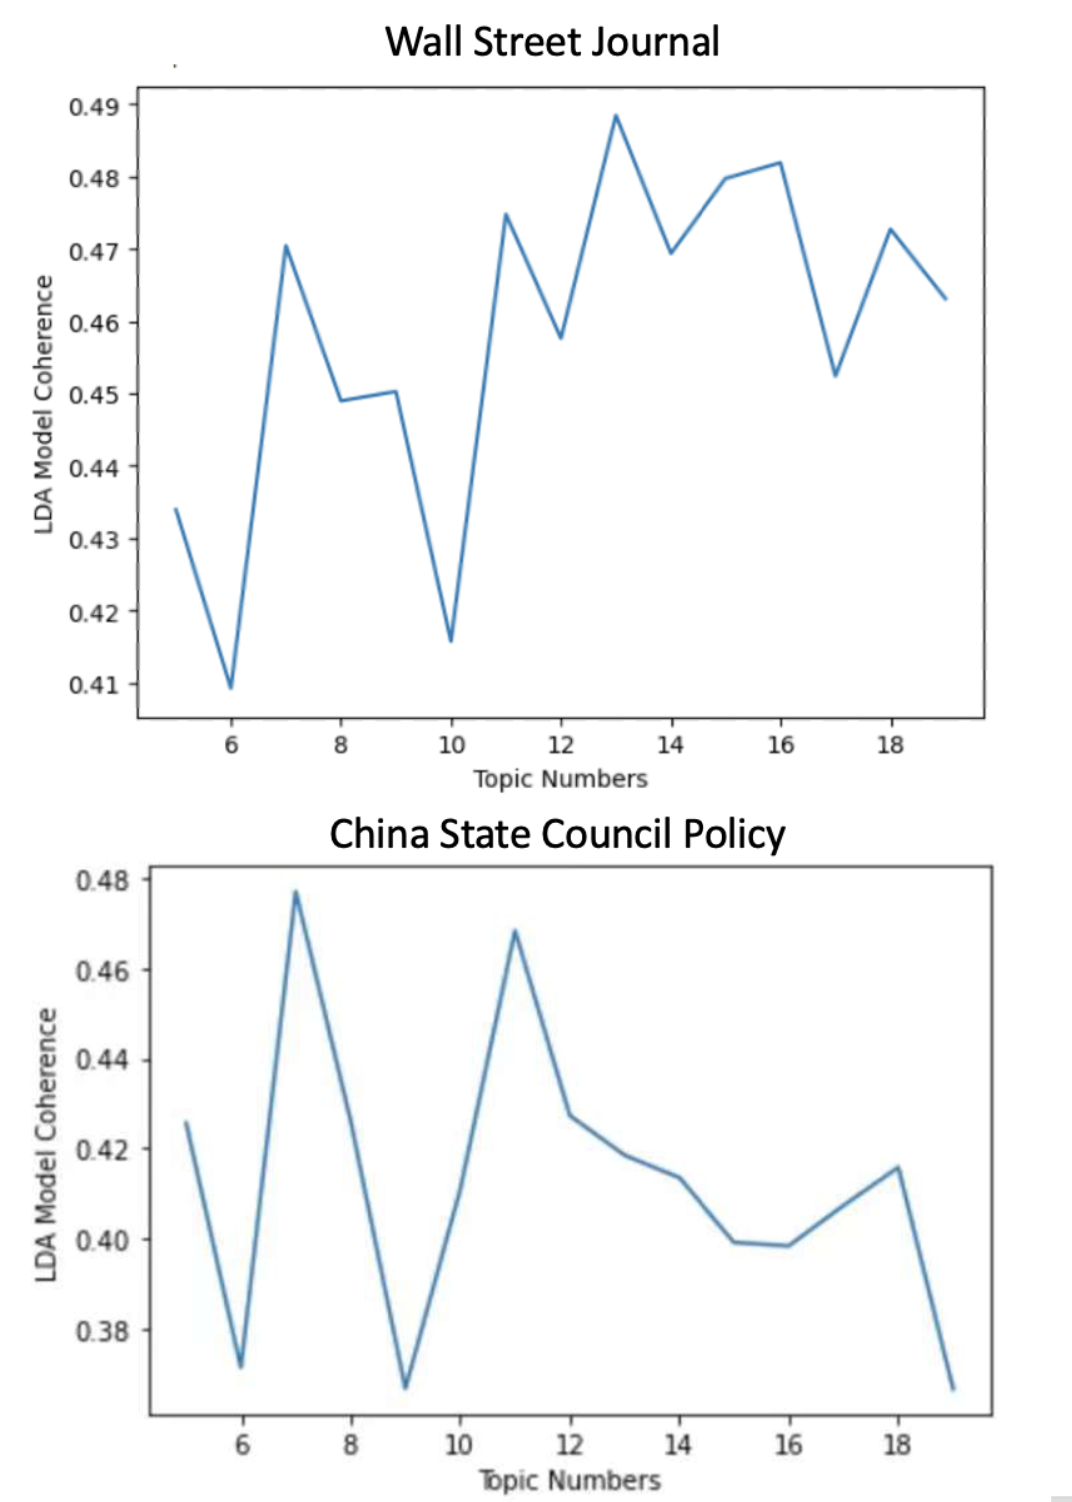
\includegraphics[width=0.8\textwidth]{fig/fig5.png}
    \caption*{Figure 5: Điểm nhất quán (Coherence) của LDA}
    \label{fig:fig2}
\end{figure}

\noindent
\subsubsection{{Ý nghĩa kết hợp dữ liệu:}}
\begin{itemize}
    \item Sử dụng dữ liệu từ cả WSJ và chính sách Trung Quốc cho phép kiểm tra khả năng của ChatGPT trong xử lý thông tin đa ngôn ngữ và đa bối cảnh.
    \item Dữ liệu chính sách Trung Quốc đặc biệt hữu ích để đánh giá khả năng của ChatGPT trong phản ứng với tin tức có tính định hướng chính sách, vốn ảnh hưởng mạnh đến thị trường chứng khoán Trung Quốc.
\end{itemize}

\noindent
\subsubsection{{Kết quả chính:}}
\begin{itemize}
    \item ChatGPT có thể đề xuất danh mục đầu tư với alpha vượt trội (tới 3\%/tháng) từ cả hai nguồn dữ liệu.
    \item Phân tích văn bản truyền thống (như cosine similarity giữa tin tức và báo cáo tài chính) không tạo ra danh mục đầu tư có alpha dương, khẳng định ưu thế của ChatGPT trong xử lý dữ liệu phi cấu trúc.
\end{itemize}
\section{Phương pháp}
Nhóm tác giả đã sử dụng một truy vấn hội thoại đơn giản và trực tiếp để trích xuất các khuyến nghị đầu tư, tương tự như cách một cá nhân sẽ giao tiếp với cố vấn đầu tư của mình. Dưới đây là mẫu prompt (câu lệnh truy vấn) được sử dụng để trích xuất khuyến nghị cổ phiếu của ChatGPT.


\subsection{Hướng dẫn khuyến nghị cổ phiếu tại Mỹ dựa trên Wall Street Journal}
Hướng dẫn khuyến nghị cổ phiếu tại Mỹ dựa trên Wall Street Journal có nội dung như sau: "Giả sử bạn là một nhà phân tích tài chính cấp cao. Vui lòng đọc kỹ bản tin Wall Street Journal sau đây. Theo nội dung của bản tin, nếu bạn có khuyến nghị cổ phiếu, hãy viết "YES" và liệt kê 5 tên cổ phiếu NYSE hoặc Nasdaq cùng với mã cổ phiếu mà bạn khuyến nghị. Nếu bạn chỉ trả lời "NO", vui lòng giải thích ngắn gọn lý do.".

\subsection{Hướng dẫn khuyến nghị ngành tại Mỹ dựa trên Wall Street Journal}
Tương tự, hướng dẫn khuyến nghị ngành tại Mỹ dựa trên Wall Street Journal được thiết lập như sau: "Giả sử bạn là một nhà phân tích tài chính cấp cao. Vui lòng đọc kỹ bản tin chính sách sau đây. Dựa trên nội dung của bản tin chính sách và tham chiếu tiêu chuẩn phân loại SIC hai chữ số, nếu bạn có khuyến nghị ngành, hãy viết "YES" và liệt kê mã danh mục của ngành được khuyến nghị. Nếu bạn chỉ trả lời "NO", vui lòng giải thích ngắn gọn lý do.".

\subsection{Ví dụ minh họa}
Phụ lục (Appendix) trình bày một ví dụ về cổ phiếu mà ChatGPT đề xuất. Cụ thể, vào ngày 14 tháng 5 năm 2023, Tạp chí Phố Wall đã xuất bản một bài báo có tiêu đề: \textit{Biden to Withhold Tariffs on Solar Imports}. Bài báo này thảo luận về những người thắng và thua từ lệnh hành pháp mới này của Biden. Nhóm tác giả đã thực hiện một vòng truy vấn khi tham số nhiệt độ được đặt là một cho ChatGPT 3.5 và ChatGPT đã khuyến nghị tổng cộng năm cổ phiếu.

\subsection{Cải thiện khả năng khuyến nghị của ChatGPT thông qua tinh chỉnh}
Tiếp theo, nhóm tác giả cải thiện khả năng khuyến nghị cổ phiếu của ChatGPT dựa trên fine-tuning (tinh chỉnh). Cụ thể, đối với Wall Street Journal, họ tiền huấn luyện ChatGPT dựa trên tập dữ liệu mẫu từ năm 2018 đến 2019. Hoặc, đối với mỗi bài báo, họ cung cấp cho ChatGPT năm cổ phiếu có hiệu suất tốt nhất với cùng mã SIC hai chữ số dựa trên khuyến nghị ban đầu, và sử dụng mẫu này để tinh chỉnh đầu ra của ChatGPT.


\subsection{Đánh giá tính hợp lý của các khuyến nghị}
Để kiểm tra xem lý do đằng sau các khuyến nghị cổ phiếu có hợp lý hay không và liệu các cổ phiếu được ChatGPT khuyến nghị có phù hợp với đánh giá của một nhà phân tích tài chính con người hay không, nhóm tác giả đã thuê các chuyên gia kỳ cựu trong ngành kết hợp với sinh viên chuyên ngành tài chính. Các nhà phân tích tài chính được thuê đã vượt qua kỳ thi CFA Level 3 và các sinh viên đã vượt qua ít nhất kỳ thi CFA Level 1.


Quy trình đánh giá bao gồm các bước sau:
\begin{itemize}
\item Thứ nhất, họ cung cấp cho những người tham gia một cái nhìn tổng quan ngắn gọn về ChatGPT và khả năng của nó trong việc tạo ra các khuyến nghị cổ phiếu dựa trên các thông báo chính sách.
\item Sau đó, họ hướng dẫn những người tham gia đánh giá các khuyến nghị và quyết định liệu khuyến nghị đó có hợp lý (logical), không rõ ràng (unclear) hay hoàn toàn không liên quan (clearly unrelated) dựa trên các tiêu chí sau:
\begin{enumerate}[label=(\alph*)]
\item Mức độ liên quan đến ngành được chỉ định trong thông báo chính sách.
\item Tính vững chắc của lý do đằng sau các khuyến nghị.
\item Các cơ hội đầu tư tiềm năng dựa trên chính sách và các cổ phiếu được khuyến nghị.
\end{enumerate}
\item Đối với mỗi khuyến nghị cổ phiếu, nhóm tác giả yêu cầu hai nhà phân tích tài chính đánh giá.
\item Nếu họ đạt được cùng một kết luận, thì kết quả tương ứng sẽ được ghi nhận trực tiếp.
\item Nếu hai nhà phân tích tài chính có ý kiến khác nhau, họ yêu cầu nhà phân tích thứ ba đưa ra một đánh giá khác, và kết quả theo đa số sẽ được chấp nhận.
\item Nếu cả ba nhà phân tích tài chính đưa ra các kết quả khác nhau, mẫu này sẽ bị loại bỏ.
\end{itemize}
Đối với 92\% mẫu, kết quả được đưa ra ngay trong vòng đầu tiên, và trong 8\% trường hợp, một nhà phân tích thứ ba được mời. Không có trường hợp nào mà nhà phân tích thứ ba đưa ra kết luận thứ ba hoàn toàn khác biệt.





\subsection{Thống kê đặc điểm cổ phiếu và bản tin chính sách}
\begin{figure}[H]
    \centering
    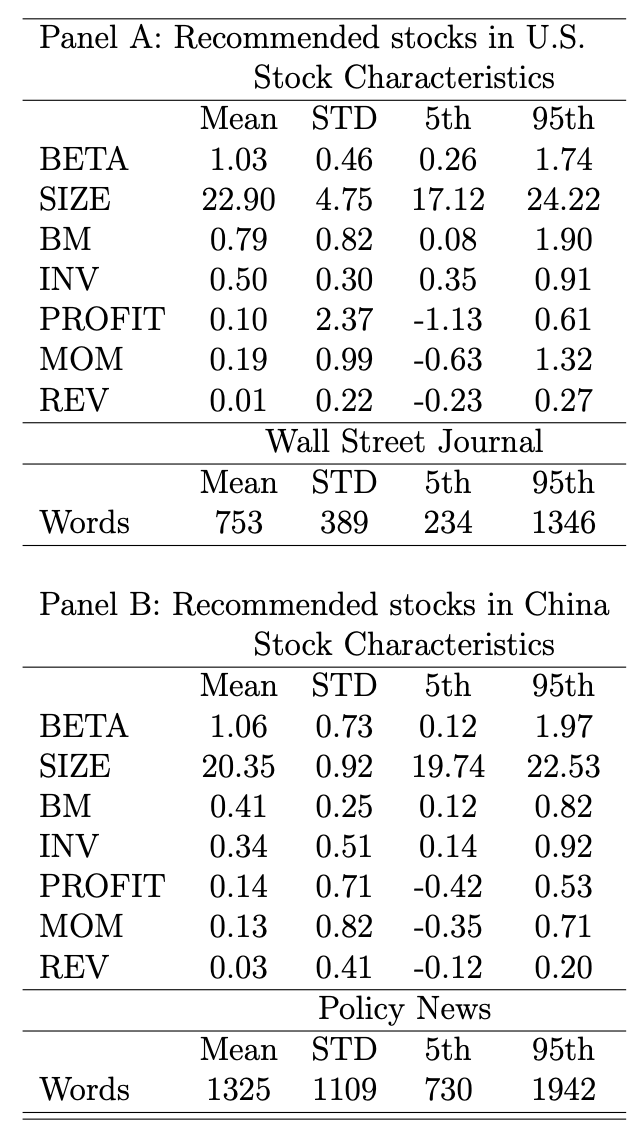
\includegraphics[width=0.5\textwidth]{table/tab1.png}
    \caption*{Table 1: Tóm tắt thống kê}
    \label{fig:tab1}
\end{figure}
Bảng 1 (Table 1) trình bày thống kê tóm tắt về đặc điểm cổ phiếu và phân bố số lượng từ trong các bài báo Wall Street Journal và các bản tin chính sách của Hội đồng Nhà nước Trung Quốc.
\begin{itemize}
\item \textbf{Panel A} hiển thị đặc điểm của cổ phiếu được ChatGPT khuyến nghị tại thị trường Hoa Kỳ và phân bố số lượng từ của các bài báo Wall Street Journal trong mẫu từ tháng 1 năm 2020 đến tháng 8 năm 2023. Các đặc điểm cổ phiếu bao gồm beta Scholes-Williams-Dimson (BETA), vốn hóa thị trường (SIZE), tỷ lệ sách trên thị trường Fama-French (BM), đầu tư (INV), lợi nhuận hoạt động (PROFIT), động lượng Jegadeesh-Titman (MOM), và đảo chiều ngắn hạn Jegadeesh-Lehmann (REV). Phân bố số lượng từ trong các bài báo Wall Street Journal được đặc trưng bởi giá trị trung bình, độ lệch chuẩn, và phần trăm vị thứ 5 và 95 của số lượng từ trên mỗi bài báo.
\item \textbf{Panel B} báo cáo đặc điểm của cổ phiếu được ChatGPT khuyến nghị tại thị trường Trung Quốc và phân bố số lượng từ trong các bản tin chính sách của Quốc vụ viện Trung Quốc trong mẫu từ tháng 1 năm 2004 đến tháng 8 năm 2023. Các đặc điểm cổ phiếu tương tự như những đặc điểm được trình bày trong Panel A, cung cấp cái nhìn sâu sắc về các cổ phiếu được khuyến nghị của thị trường Trung Quốc. Phân bố số lượng từ của các bản tin chính sách của Quốc vụ viện Trung Quốc cũng được tóm tắt bằng giá trị trung bình, độ lệch chuẩn, và phần trăm vị thứ 5 và 95 của số lượng từ trên mỗi bản tin.
\end{itemize}
\begin{figure}[H]
    \centering
    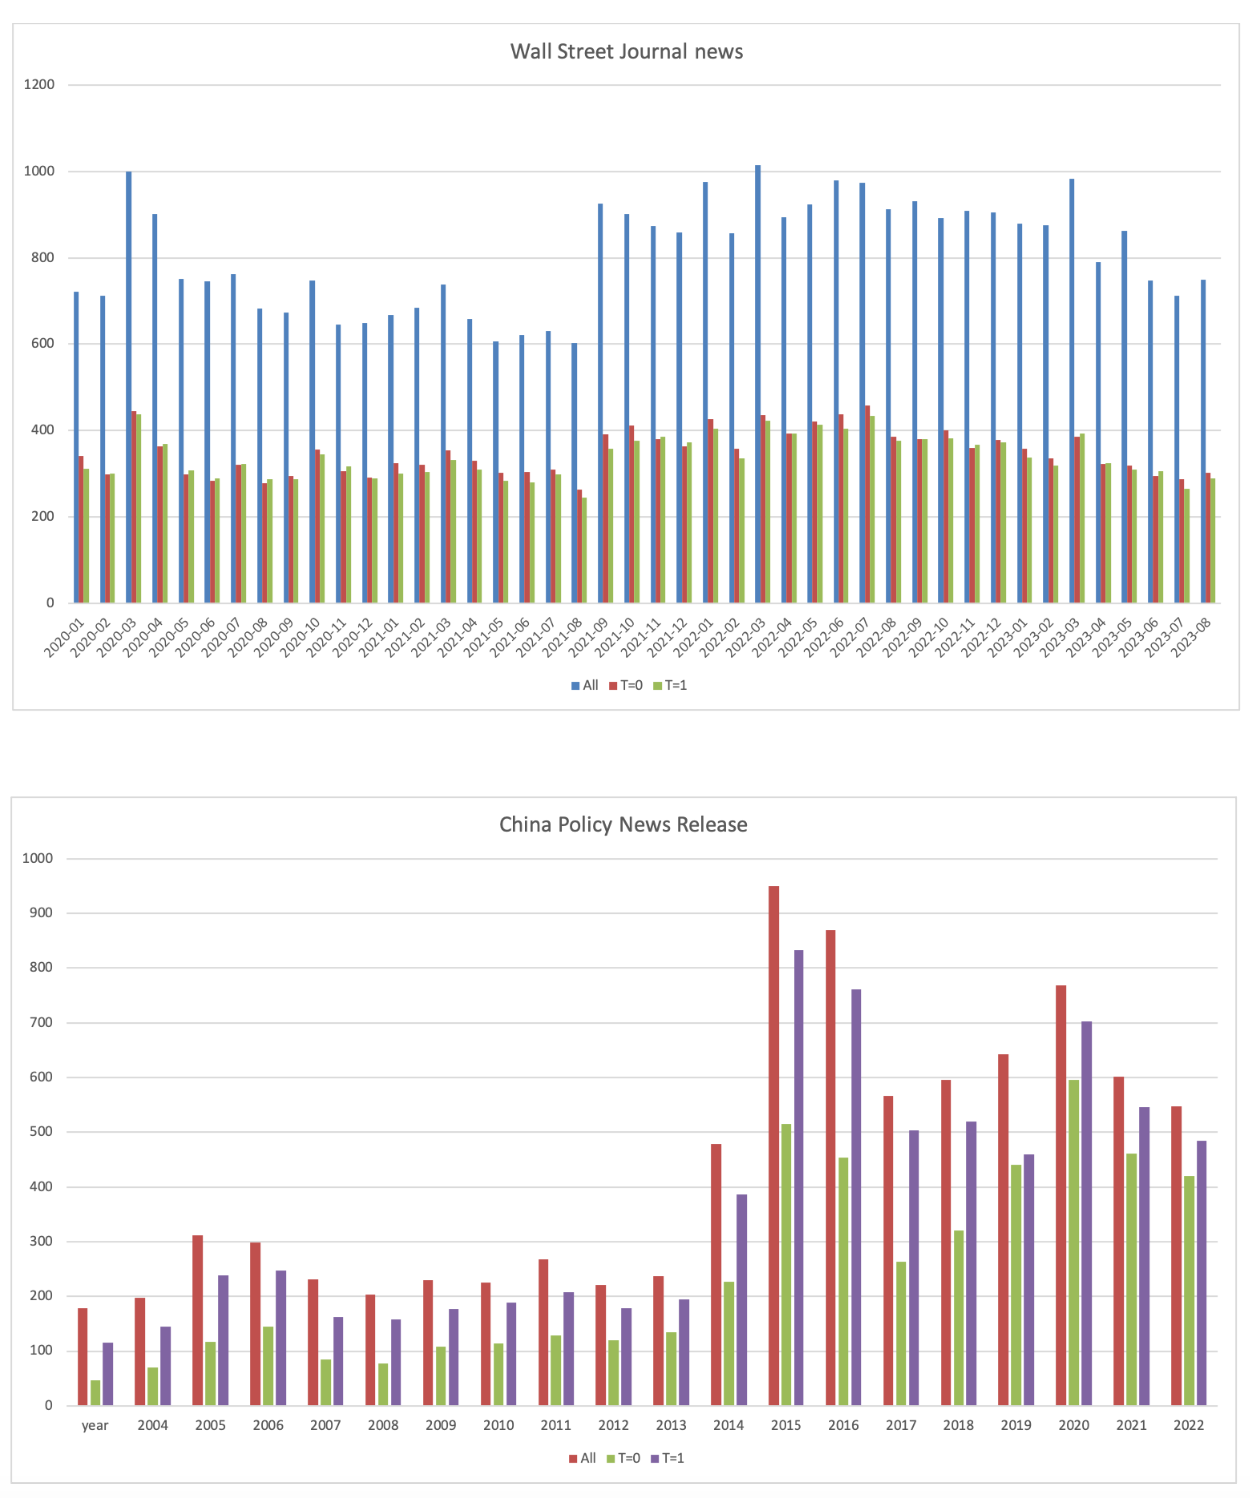
\includegraphics[width=0.8\textwidth]{fig/fig2.png}
    \caption*{Figure 2: Số lượng báo cáo phát hành chính sách trong chuỗi thời gian}
    \label{fig:fig2}
\end{figure}
Hình 2 (Figure 2) hiển thị số lượng bản tin chính sách được phát hành theo năm trong giai đoạn mẫu của nghiên cứu, với tổng số hơn 20.000 bản tin Wall Street Journal. ChatGPT nhận thấy khoảng dưới một nửa số bản tin chính sách này có liên quan đến khuyến nghị cổ phiếu theo chuỗi thời gian. Kết quả này không thay đổi nhiều tùy theo tham số nhiệt độ được đặt. Nhìn chung, các thống kê tóm tắt này làm nổi bật sự đa dạng về cả đặc điểm cổ phiếu và nội dung tin tức chính sách, điều này cung cấp một bối cảnh phong phú cho phân tích của nhóm tác giả

\section{Testing ChatGPT sử dụng dữ liệu chính sách của Mỹ}

\subsection{Kiểm tra lập luận dựa trên đánh giá của con người}
Trong phần này, nhóm nghiên cứu tiến hành kiểm tra khả năng lập luận của ChatGPT trong việc đưa ra khuyến nghị đầu tư dựa trên nội dung chính sách tại Mỹ (Wall Street Journal). Do số lượng lớn các tin tức chính sách và khuyến nghị cổ phiếu, nhóm nghiên cứu đã lựa chọn ngẫu nhiên 100 mẫu tin tức chính sách cho mỗi lần kiểm tra.
\\ Mỗi khuyến nghị đầu tư được đánh giá theo ba tiêu chí:\begin{itemize}
    \item Tính liên quan (Relevance)
    \item Lý do hợp lý (Reasoning)
    \item Co hội đầu tư (Investment Opportunity)
\end{itemize}

Kết quả đánh giá được phân loại thành 3 nhóm:

\begin{itemize}
    \item Hợp lý (Logical)
    \item Không rõ ràng (Unclear)
    \item Không liên quan (Unrelated)
\end{itemize}
Kết quả kiểm tra được tổng hợp trong \textbf{Bảng 2} với hai bảng con: 
\begin{figure}[H]
    \centering
    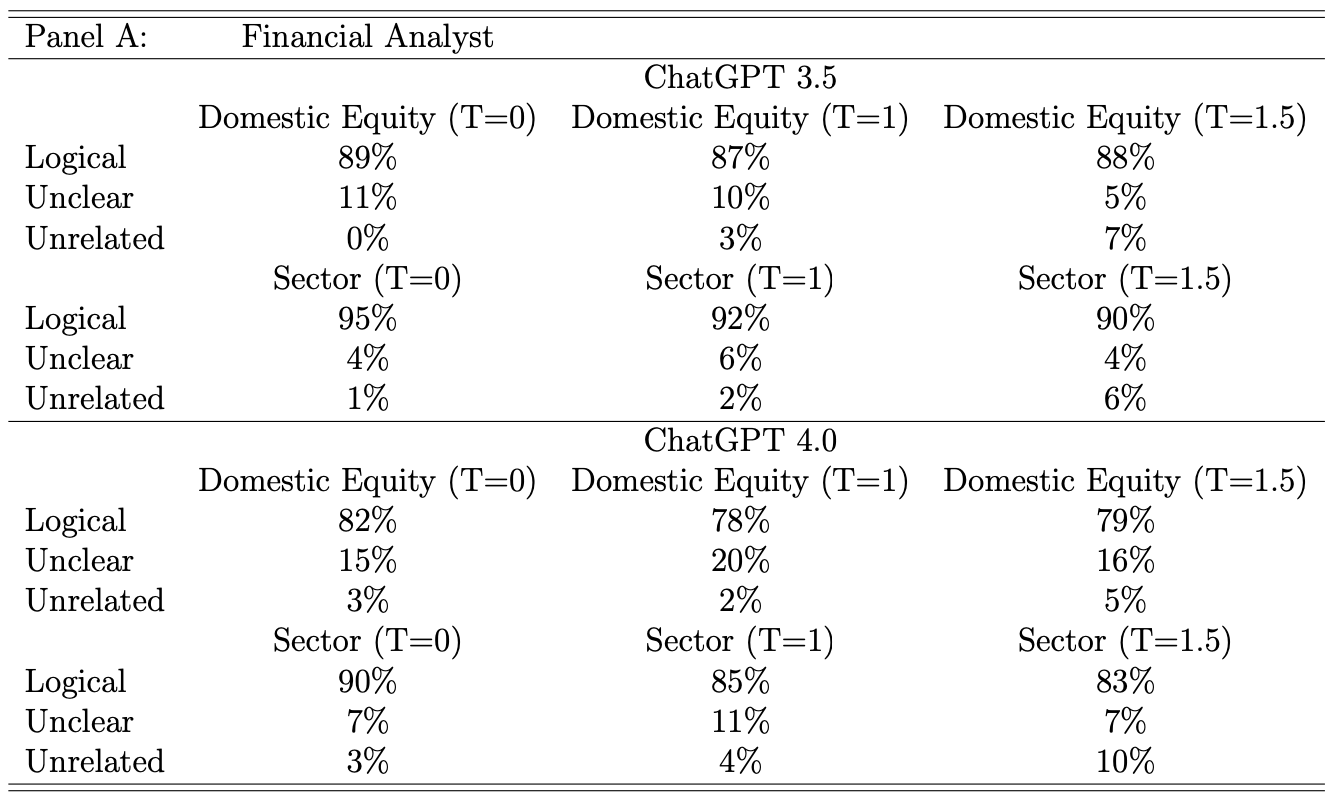
\includegraphics[width=0.8\textwidth]{table/tab2a.png}
    \caption*{Table 2a: Tư vấn đầu tư của ChatGPT và tính hợp lệ tại Mỹ}
    \label{fig:fig2}
\end{figure}
\begin{figure}[H]
    \centering
    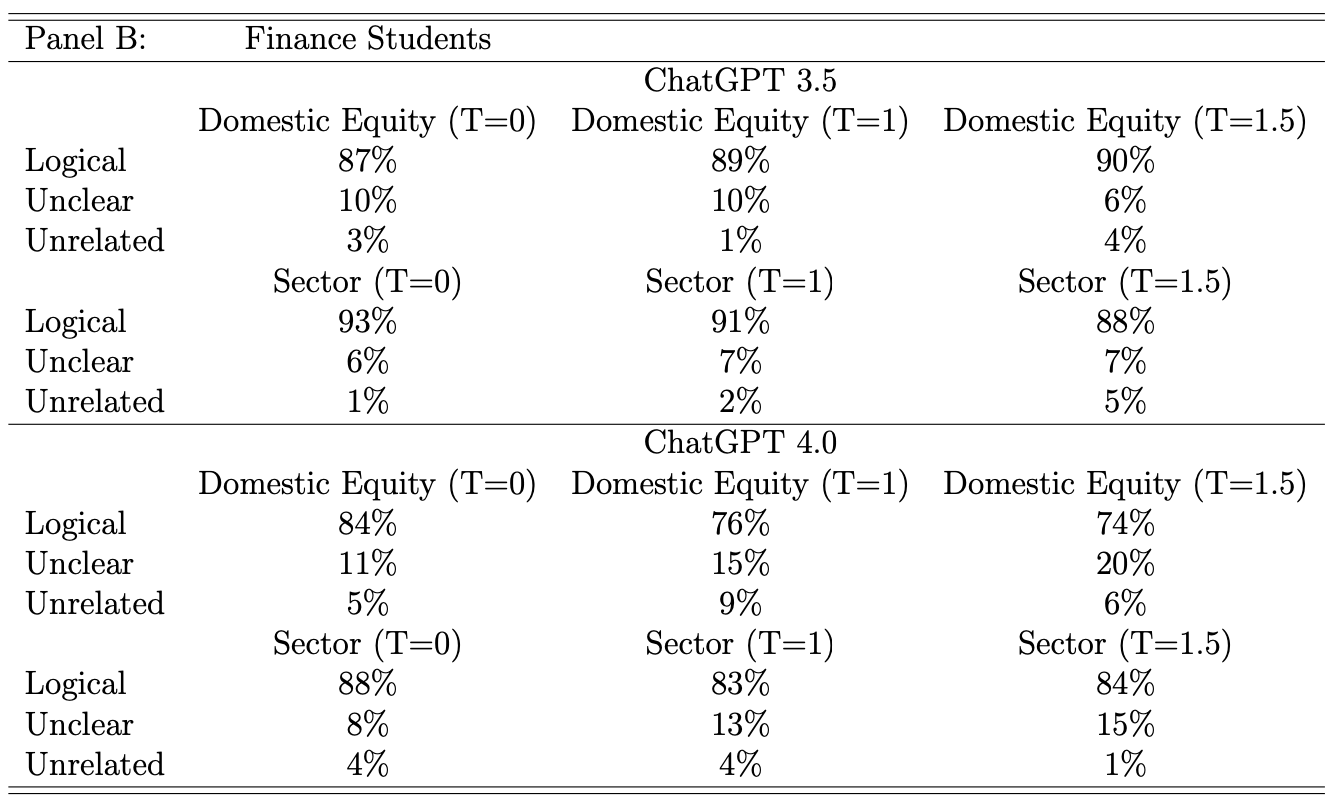
\includegraphics[width=0.8\textwidth]{table/tab2b.png}
    \caption*{Table 2b: Tư vấn đầu tư của ChatGPT và tính hợp lệ tại Mỹ (tiếp theo)}
    \label{fig:fig2}
\end{figure}
\textbf{(a)} kết quả đánh giá của nhóm chuyên gia tài chính, và \textbf{(b)} kết quả đánh giá của nhóm sinh viên chuyên ngành tài chính. Ngoài ra, nghiên cứu cũng phân tích tác đồng của tham số nhiệt độ (\textbf{Temperature parameter T}) của ChatGPT - một tham số điều chỉnh mức độ sáng tạo trong phản hồi của mô hình. Cụ thể, ba giá trị nhiệt độ được sử dụng: \textbf{T = 0, T = 1, T = 1.5}. Mỗi giá trị này được áp dụng cho 2 nhóm khuyến nghị: \textbf{Domestic Equity} (khuyến nghị cổ phiếu riêng lẻ trên NYSE hoặc Nasdaq) và \textbf{Sector} (khuyến nghị ngành dựa trên mã ngành SIC hai chữ số).
\\ 
\textbf{Kết quả:}\begin{itemize}
    \item Kết quả cho thấy, trong nhóm Domestic Equity, tỷ lệ khuyến nghị hợp lý dao động từ 74\% đến 90\%, tùy thuộc vào nhóm người đánh giá và mức nhiệt độ. Đối với nhóm Sector, tỷ lệ hợp lý cao hơn, dao động từ 83\% đến 95\%, cho thấy ChatGPT có khả năng đưa ra khuyến nghị ngành tốt hơn so với khuyến nghị cổ phiếu riêng lẻ.
    \item So sánh giữa ChatGPT 3.5 và ChatGPT 4.0, kết quả cho thấy ChatGPT 3.5 thường có tỷ lệ khuyến nghị hợp lý cao hơn so với ChatGPT 4.0 ở cả hai nhóm đánh giá và trong cả hai nhóm khuyến nghị. Ví dụ, trong nhóm Domestic Equity với T=0, tỷ lệ khuyến nghị được đánh giá là hợp lý bởi chuyên gia tài chính là 89\% đối với ChatGPT 3.5, trong khi ChatGPT 4.0 chỉ đạt 82\%. Xu hướng tương tự cũng xuất hiện trong đánh giá của sinh viên chuyên ngành tài chính.
\end{itemize}
\noindent
\\ Tóm lại, kết quả từ \textbf{Bảng 2} chỉ ra rằng khuyến nghị đầu tư của ChatGPT phần lớn là được đánh giá \textbf{hợp lý} đối với cả ChatGPT 3.5 và ChatGPT 4.0, trong đó hai nhóm Domestic Equity và Sector. Tỷ lệ khuyến nghị \textbf{không rõ ràng} và \textbf{không liên quan} đều thấp, cho thất \textbf{tiềm năng của ChatGPT như một công cụ hỗ trợ tư vấn đầu tư}.

\subsection{Thị trường chứng khoán Mỹ:Kiểm định trong mẫu (In-sample test)}
\subsubsection{Mục tiêu và thiết kế nghiên cứu}
Phần kiểm định trong mẫu (In-sample test) được thiết kế nhằm đánh giá khả năng của mô hình ChatGPT trong việc tạo ra các danh mục cổ phiếu có hiệu suất vượt trội, dựa trên việc phân tích văn bản tài chính phi cấu trúc. Trong trường hợp này, dữ liệu văn bản được lấy từ các bài viết trên \textbf{Wall Street Journal (WSJ)}- một nguồn tin uy tín về tài chính và kinh doanh - trong giai đoạn từ \textbf{tháng 1 năm 2020 đến tháng 8 năm 2021}. Đây là khoảng thời gian được cho là nằm \textbf{trong đợt tập huấn luyện của ChatGPT}, nên mô hình có thể đã tiếp xúc với những dữ liệu này trong quá trình pre-training, từ đó có thể biểu hiện tốt hơn so với dữ liệu hoàn toàn mới (out-of-sample)
\\ Để kiểm định một cách hệ thống, nhóm tác giả thực hiện các bước sau:
\begin{enumerate}
    \item \textbf{Tiền xử lý dữ liệu}\begin{itemize}
        \item Chọn lọc các bài viết WSJ có liên quan đến tài chính hoặc kinh tế vĩ mô.
        \item Mỗi bài viết được dùng để tạo một \textbf{prompt} đầu vào cho ChatGPT, yêu cầu mô hình \textbf{đề xuất 5 cổ phiếu cụ thể} nên mua dựa trên nội dung của bài viết đó.
        \item Dữ liệu được chuẩn hoá để mô phỏng cách nhà đầu tư tương tác với một "robo-advisor AI"
    \end{itemize}
    \item \textbf{Tạo danh mục đầu tư theo lịch trình} : Sau khi ChatGPT đưa ra danh sách cổ phiếu, các \textbf{danh mục đầu tư (portfolio)} được xây dựng dựa trên mô hình \textbf{calendar-time}:\begin{itemize}
        \item Mỗi ngày (hoặc tuần/tháng) trong giai đoạn kiểm định, hệ thống sẽ xây dựng một danh mục mới dựa trên phản hồi từ CHatGPT cho các bài viết WSJ ngày hôm đó.
        \item Các danh mục có thời gian nắm giữ cố định: 1 ngày, 1 tuần, 1 tháng và 3 tháng.
        => Điều này mô phỏng tình huống thực tế nơi nhà đầu tư liên tục nhận được các đề xuất mới từ AI và duy trì các khoản đầu tư theo thời hạn đã định
    \end{itemize}
    \item \textbf{Trọng số danh mục và biến thể đầu tư}: Hai phương pháp gán trọng số cho cổ phiếu trong danh mục được áp dụng \begin{itemize}
        \item \textbf{Equal-weighted (EW)}: Mỗi cổ phiếu có trọng số bằng nhau
        \item  \textbf{Value-weighted (VW)}: Trọng số theo vốn hoá thị trường
        => Điều này nhằm kiểm tra xem hiệu quả của ChatGPT có phụ thuộc vào cách gán trọng số hay không.
    \end{itemize}
    \item \textbf{Kiểm định thống kê bằng mô hình định giá tài sản}: Lợi nhuận của các danh mục được đánh giá bằng \textbf{mô hình hồi quy theo thời gian} (time-series regression) với cấc mô hình định giá phổ biến \begin{itemize}
        \item \textbf{CAPM}: kiểm tra alpha so với chỉ số thị trường
        \item  \textbf{Fama-Fench 3 yếu tố (FF3)}: thêm yếu tố quy mô (SMB) và giá trị HML
        \item \textbf{Fama-Fench 5 yếu tố (FF5)}: thêm yếu tố lợi nhuận và đầu tư
        \item \textbf{FF5 + MOM + REV}: thêm yếu tố đà tăng (momentum) và đảo chiều ngắn hạn (reversal).
        \\=>\textbf{Hệ số alpha} (lợi nhuận vượt trội điều chỉnh theo rủi ro) là tiêu chí đánh giá chính. Nếu alpha dương và có ý nghĩa thống kê, ChatGPT được xem là tạo ra danh mục đầu tư có giá trị thực sự.
    \end{itemize}
    \item \textbf{Biến thể về tham số ChatGPT: Temperature}: Hai thiết lập của tham số \textbf{temperature} trong ChatGPT được so sánh: \begin{itemize}
        \item \textbf{T = 0}: phản hồi nhất quán, bảo thủ (giống một chuyên gia cố định)
        \item \textbf{T = 1}: phản hồi đa dạng, sáng tạo (giống nhiều chuyên gia khác nhau). Đặc biệt khi \textbf{T = 1}, mỗi danh mục được toạ thành từ tất cả các cổ phiếu được Chat GPT đề xuất qua 25 lần truy vấn khác nhau, nhằm tận dụng sư đa dạng trong phản hồi của mô hình.
        \\=> Mục tiêu là kiểm tra xem sự ngẫu nhiên và đa dạng trong phản hồi có giúp tăng khả năng tạo lợi nhuận hay không.
    \end{itemize}

\end{enumerate}
\subsubsection{Kết quả kiểm tra trong mẫu}
\begin{figure}[H]
    \centering
    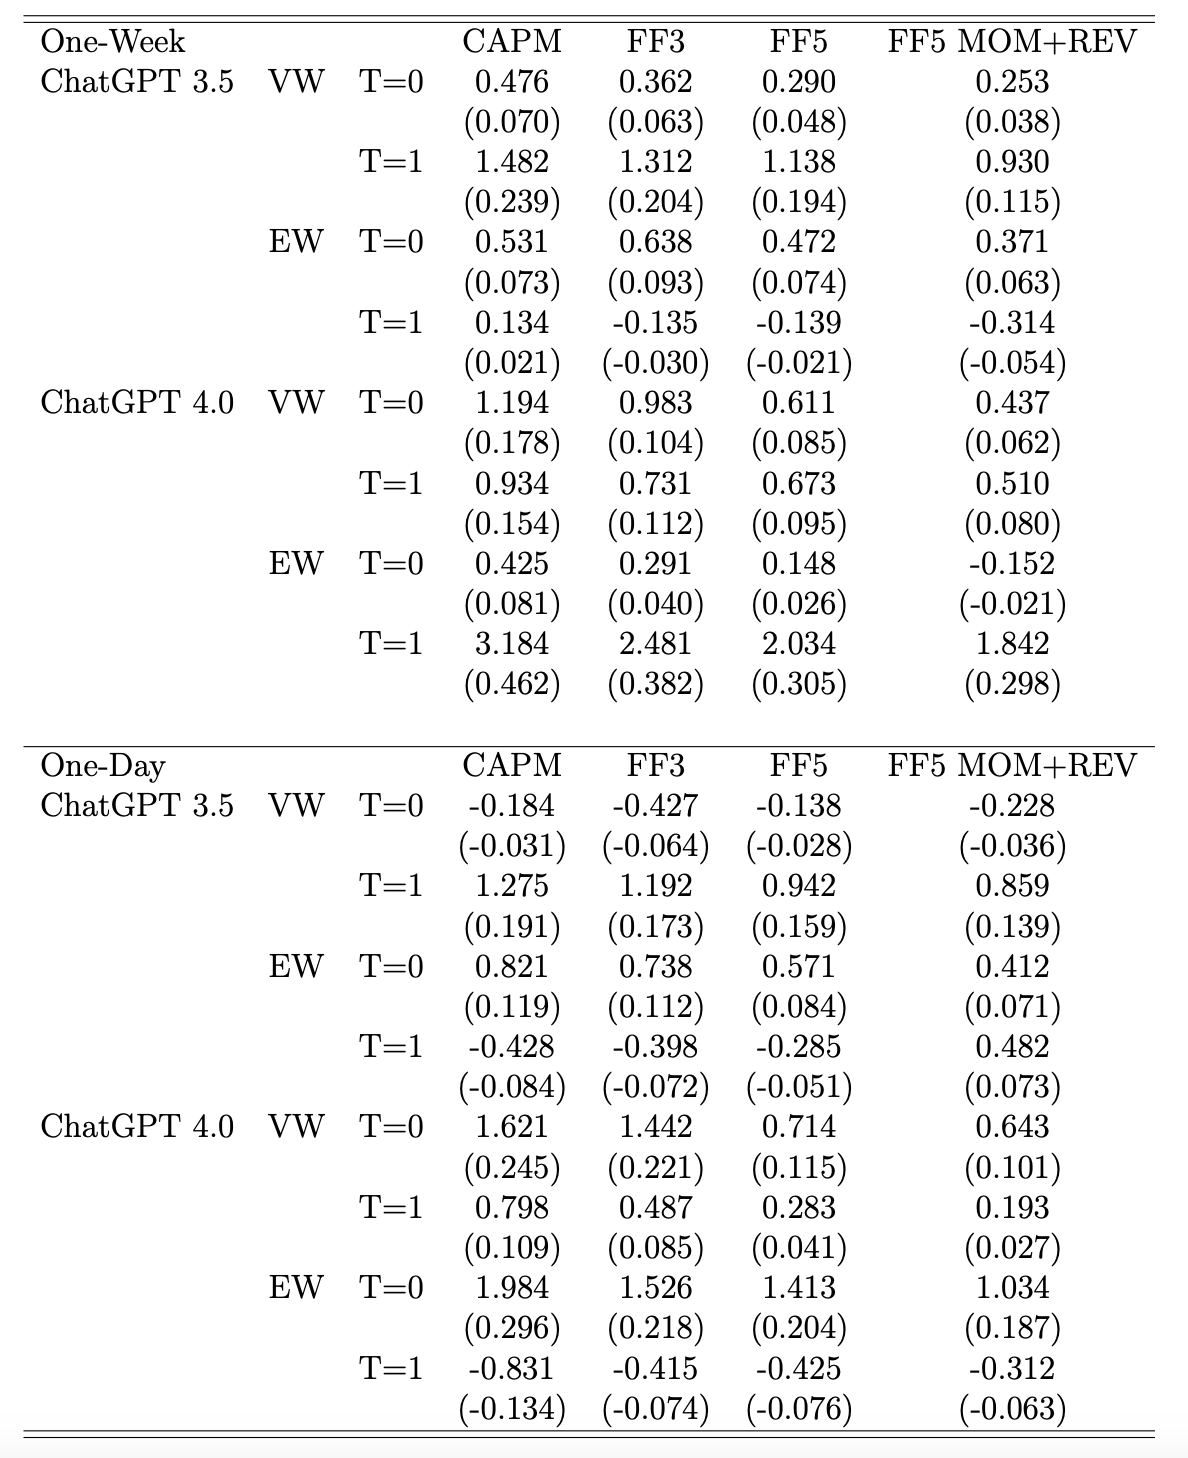
\includegraphics[width=0.8\textwidth]{table/tab3b.png}
    \label{fig:fig2}
\end{figure}
\begin{figure}[H]
    \centering
    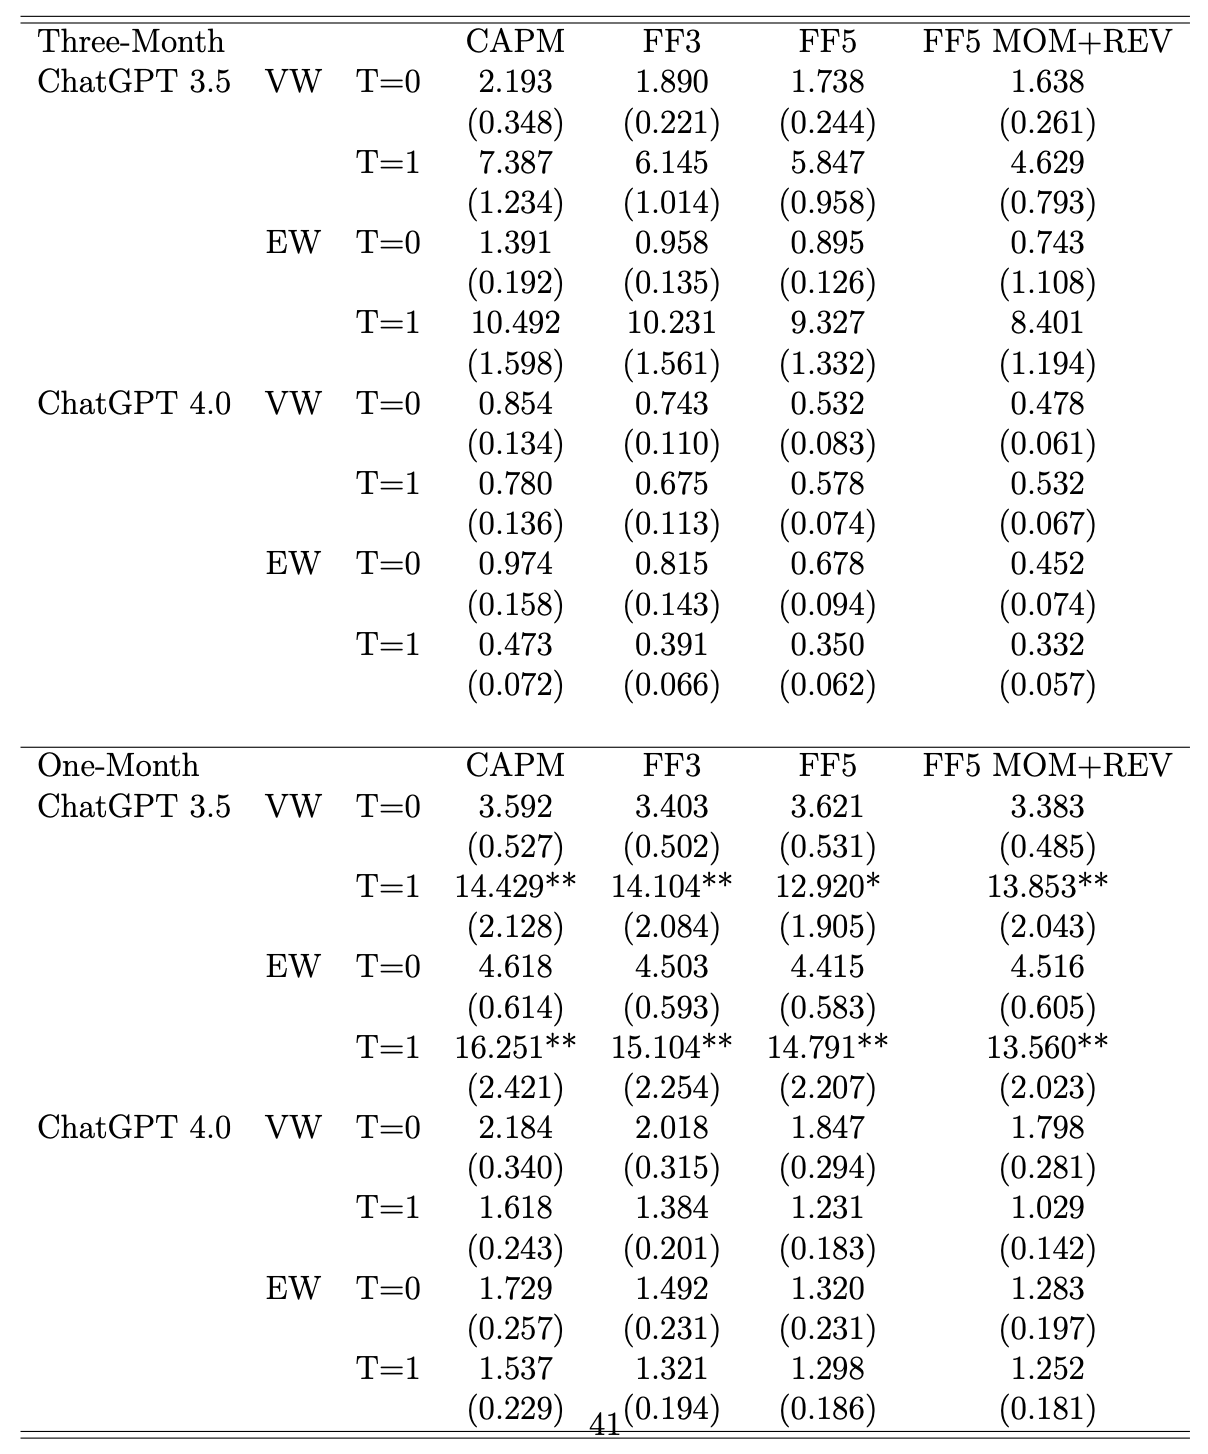
\includegraphics[width=0.8\textwidth]{table/tab3a.png}
    \caption*{Table 3: Alphas của Cổ phiếu được Đề xuất dựa trên Wall Street Journal: In-sample test}
    \label{fig:fig2}
\end{figure}
Kết quả được trình bày trong \textbf{Bảng 3}, cho thấy hiệu suất của các danh mục đầu tư dựa trên các chỉ số alpha hàng ngày (daily alpha) và thống kê t (t-statistics).
\begin{itemize}
    \item \textbf{So sánh ChatGPT 3.5 và 4.0:}
    \\Trong hầu hết các khoảng thời gian nắm giữ và mô hình yếu tố, \textbf{ChatGPT 3.5 cho thấy hiệu suất cao hơn ChatGPT 4.0}, với các giá trị alpha cao hơn và thống kê t lớn hơn. Ví dụ, ở khoảng thời gian \textbf{3 tháng}, danh mục VW của ChatGPT 3.5 có alpha theo mô hình CAPM là \textbf{2.193}, trong khi của ChatGPT 4.0 chỉ đạt \textbf{0.854}
    \item \textbf{Ảnh hưởng của tham số nhiệt độ}:
    \\ Hiệu suất của danh mục đầu tư thay đổi theo mức T. Cụ thể, trong khoảng thời gian \textbf{1 tháng}, alpha của ChatGPT 3.5 cho danh mục VW tăng từ \textbf{3.592 (T = 0)} lên \textbf{14.429 (T = 1)}, cho thấy sức sáng tạo cao hơn có thể mang lại lợi nhuận lớn hơn. Tuy nhiên, tác động của T không đồng nhất ở các khoảng thời gian khác, và không có mức T nào là tối ưu cho mọi trường hợp.
    \item \textbf{Hiệu suất theo khoảng thời gian nắm giữ}
    \\Kết quả chỉ ra rằng \textbf{khoảng thời gian nắm giữ 1 tháng là tối ưu}, với alpha cao nhất và ổn định hơn so với các khoảng thời gian khác (3 tháng, 1 tuần, 1 ngày). Lý do có thể là nội dung của Wall Street Journal thường mang tính ngắn hạn và thời sự, tác động mạnh đến giá cổ phiếu trong ngắn hạn.
\end{itemize}
\subsubsection{Kết luận}
Nhìn chung, \textbf{ChatGPT 3.5 vượt trội hơn ChatGPT 4.0} về khả năng đưa ra khuyến nghị đầu tư có lợi nhuận dựa trên nội dung Wall Street Journal. Hiệu suất phụ thuộc vào mô hình yếu tố, khoảng thời gian nắm giữ và mức sáng tạo T, với thời gian nắm giữ 1 tháng được xác định là tốt nhất để tối ưu hóa lợi nhuận từ khuyến nghị của ChatGPT.
\subsection{Thị trường chứng khoán Mỹ: Kiểm định ngoài mẫu  (Out-of sample test)}

\subsubsection{Giới thiệu}
Do \textbf{ChatGPT 3.5 thể hiện khả năng lý luận tốt hơn} so với ChatGPT 4.0, chúng tôi chủ yếu sử dụng \textbf{ChatGPT 3.5} để tiến hành phân tích ngoài mẫu (out-of-sample) về hiệu suất danh mục đầu tư dựa trên nội dung \textit{Wall Street Journal}. Trong phần này, khoảng thời gian nắm giữ cổ phiếu được khuyến nghị được đặt là \textbf{một tháng dương lịch} để phản ánh tác động ngắn hạn của tin tức.

\subsubsection{Phương pháp kiểm tra}
\begin{itemize}
    \item \textbf{Mô hình đánh giá}: Sử dụng mô hình Fama-French năm yếu tố (FF5), bao gồm cả các yếu tố \textbf{Động lực (Momentum)} và \textbf{Đảo ngược (Reversal)}.
    \item \textbf{Tham số nhiệt độ (T)}: Được sử dụng để điều chỉnh mức độ sáng tạo trong phản hồi của ChatGPT. Hai mức nhiệt độ được so sánh: \textbf{T=0} (ít sáng tạo) và \textbf{T=1} (nhiều sáng tạo).
    \item \textbf{Phương pháp trọng số danh mục}: Xem xét cả \textbf{trọng số đồng đều (Equal-Weighted, EW)} và \textbf{trọng số theo giá trị (Value-Weighted, VW)}.
    \item \textbf{Lợi nhuận danh mục}: Lợi nhuận được điều chỉnh theo thang điểm cơ bản (bps) và chuẩn hóa trên cơ sở 10.000.
\end{itemize}

\subsubsection{Kết quả ngoài mẫu}
Kết quả được trình bày trong \textbf{Bảng 5}, bao gồm alpha tổng thể và alpha theo từng \textbf{13 chủ đề} được xác định từ phân tích LDA.
\begin{figure}[H]
    \centering
    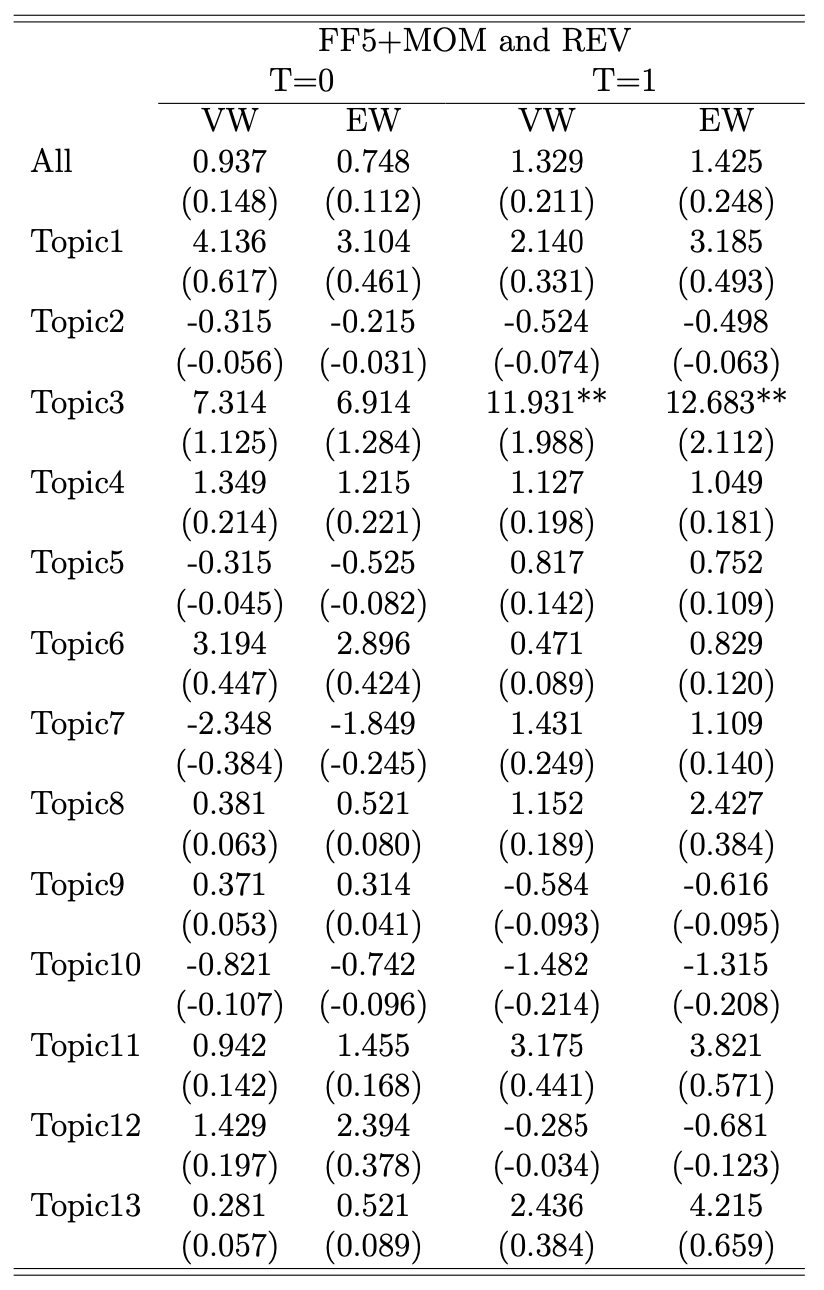
\includegraphics[width=0.5\textwidth]{table/tab5.png}
    \caption*{Table 5: Alphas của Cổ phiếu được Đề xuất dựa trên Wall Street Journal:: Out-sample test}
    \label{fig:fig2}
\end{figure}
\begin{itemize}
    \item \textbf{Kết quả tổng thể}: Khi \textbf{T=0}, các alpha của danh mục thường \textbf{dương nhưng không có ý nghĩa thống kê}, cho thấy rằng ChatGPT không tạo ra lợi nhuận vượt trội một cách nhất quán trong thời gian ngoài mẫu. Tuy nhiên, khi tăng mức sáng tạo lên \textbf{T=1}, alpha trở nên \textbf{dương hơn và có ý nghĩa thống kê} cho cả EW và VW. Điều này chỉ ra rằng mức độ sáng tạo cao hơn trong khuyến nghị của ChatGPT có thể cải thiện hiệu suất ngoài mẫu.
    \item \textbf{Hiệu suất theo chủ đề}: Hiệu suất ngoài mẫu của ChatGPT thay đổi theo từng chủ đề. \\
    \textbf{Chủ đề 3 (liên quan đến chính trị)} thể hiện alpha mạnh và có ý nghĩa thống kê ở cả hai mức nhiệt độ và hai phương pháp trọng số. Các từ khóa phổ biến trong chủ đề này bao gồm ``đảng Dân chủ'', ``đảng Cộng hòa'', ``hạ viện'', ``Biden'', ``thượng viện'' và ``bầu cử''. Danh mục đầu tư của ChatGPT có \textbf{alpha hàng ngày 11 bps}, tương đương \textbf{alpha hàng tháng 2.2\%} cho chủ đề này.\\
    Ngược lại, \textbf{Chủ đề 2} và \textbf{Chủ đề 10} cho thấy \textbf{alpha tiêu cực và không có ý nghĩa}, chứng tỏ rằng các khuyến nghị của ChatGPT cho những chủ đề này không tạo ra lợi nhuận vượt trội đồng nhất.
\end{itemize}

\subsubsection{Kết luận}
Kết quả trong \textbf{Bảng 5} cho thấy rằng \textbf{hiệu suất ngoài mẫu của ChatGPT không đồng nhất} giữa các chủ đề và mức nhiệt độ. \textbf{Mức sáng tạo cao hơn (T=1)} có xu hướng mang lại kết quả tốt hơn, đặc biệt là đối với các chủ đề liên quan đến \textbf{chính trị}. Tuy nhiên, hiệu suất tổng thể không phải lúc nào cũng có ý nghĩa thống kê, cho thấy vẫn cần thận trọng khi sử dụng khuyến nghị của ChatGPT trong thực tế đầu tư.
\subsection{Thị trường chứng khoán Mỹ: Kết quả sau khi tinh chỉnh mô hình (Fine-tuning)}

\subsubsection{Giới thiệu và phương pháp}
Phần này trình bày kết quả thử nghiệm ngoài mẫu (out-of-sample) cho danh mục đầu tư cổ phiếu được khuyến nghị dựa trên nội dung từ \textit{Wall Street Journal}, sau khi áp dụng \textbf{quy trình tinh chỉnh (fine-tuning)} cho mô hình ChatGPT.
\begin{itemize}
    \item \textbf{Mô hình}: Fama-French 5 yếu tố (FF5), bổ sung yếu tố \textbf{Động lực (MOM)} và \textbf{Đảo ngược (REV)}.
    \item \textbf{Danh mục}: Cả \textbf{Equal-Weighted (EW)} và \textbf{Value-Weighted (VW)}, trên toàn bộ tập dữ liệu và 13 chủ đề riêng lẻ.
    \item \textbf{Tham số nhiệt độ (T)}: Được xem xét tại \textbf{T=1}, tăng mức sáng tạo.
\end{itemize}

\subsubsection{Kết quả thử nghiệm}
Kết quả chi tiết được trình bày trong \textbf{Bảng 6}.
\begin{figure}[H]
    \centering
    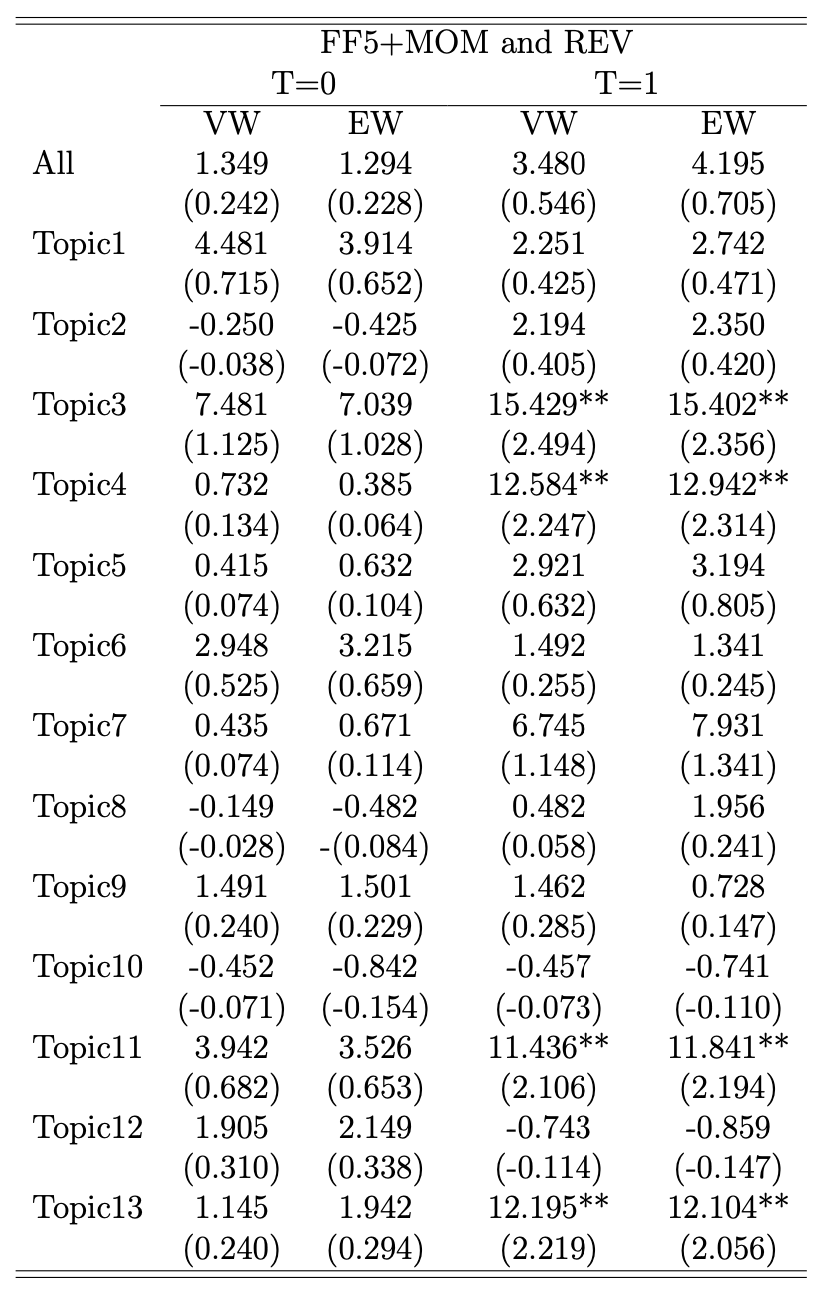
\includegraphics[width=0.5\textwidth]{table/tab6.png}
    \caption*{Table 6: Alphas của Cổ phiếu được Đề xuất dựa trên Wall Street Journal}
    \label{fig:fig2}
\end{figure}
\begin{itemize}
    \item \textbf{Tổng quan}: Khi T=1, alpha của danh mục đều dương nhưng không có ý nghĩa thống kê, với VW đạt \textbf{3.480}, EW đạt \textbf{4.195}. Điều này cho thấy, sau tinh chỉnh, danh mục vẫn tạo lợi nhuận bất thường nhưng chưa đủ mạnh để khẳng định chắc chắn.
    \item \textbf{Phân tích theo chủ đề}:
    \begin{itemize}
        \item \textbf{Chủ đề 3 (chính trị)}: Alpha mạnh và có ý nghĩa. Tại T=0, VW \textbf{7.481}, EW \textbf{7.039}; T=1, VW \textbf{15.429}, EW \textbf{15.402}, có ý nghĩa ở mức 5\%.
        \item \textbf{Chủ đề 4 (Covid-19 và Trung Quốc)}: T=0, VW \textbf{0.732}, EW \textbf{0.385} (không có ý nghĩa); T=1, VW \textbf{7.584}, EW \textbf{8.942}, có ý nghĩa ở mức 5\% và 1\%.
        \item \textbf{Chủ đề 13 (Nga-Ukraine)}: T=0, VW \textbf{1.145}, EW \textbf{1.942} (không có ý nghĩa); T=1, VW \textbf{12.195}, EW \textbf{12.104}, có ý nghĩa ở mức 5\%.
    \end{itemize}
\end{itemize}

\subsubsection{So sánh với phân tích văn bản truyền thống}
\begin{figure}[H]
    \centering
    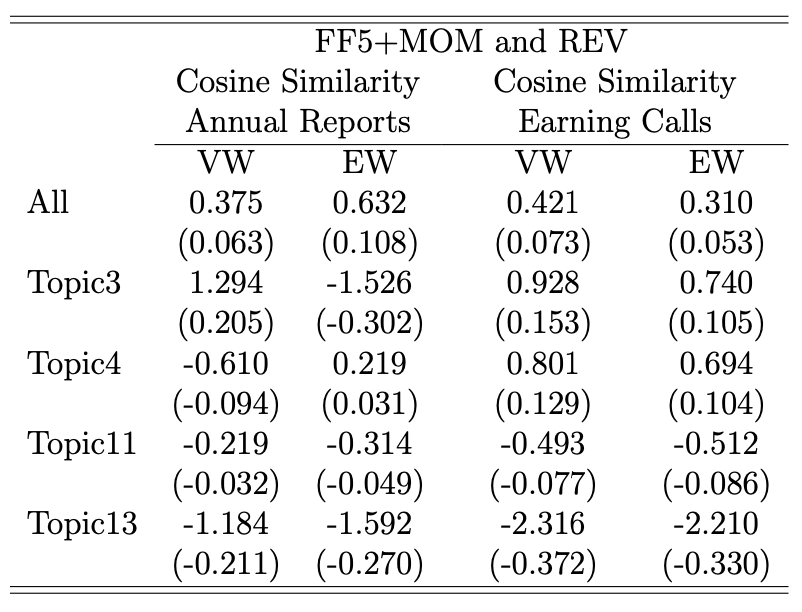
\includegraphics[width=0.6\textwidth]{table/tab7a.png}
    \caption*{Table 7: Phân tích của Wall Street Journal so sánh với phân tích văn bản truyền thống}
    \label{fig:fig2}
\end{figure}
\textbf{Bảng 7} cho thấy ChatGPT vượt trội so với phương pháp phân tích văn bản truyền thống (dựa trên tương tự cosine) ở các chủ đề 3, 4 và 13, chứng minh ưu thế của học máy.

\subsubsection{Kết quả trực quan hóa}
\begin{figure}[H]
    \centering
    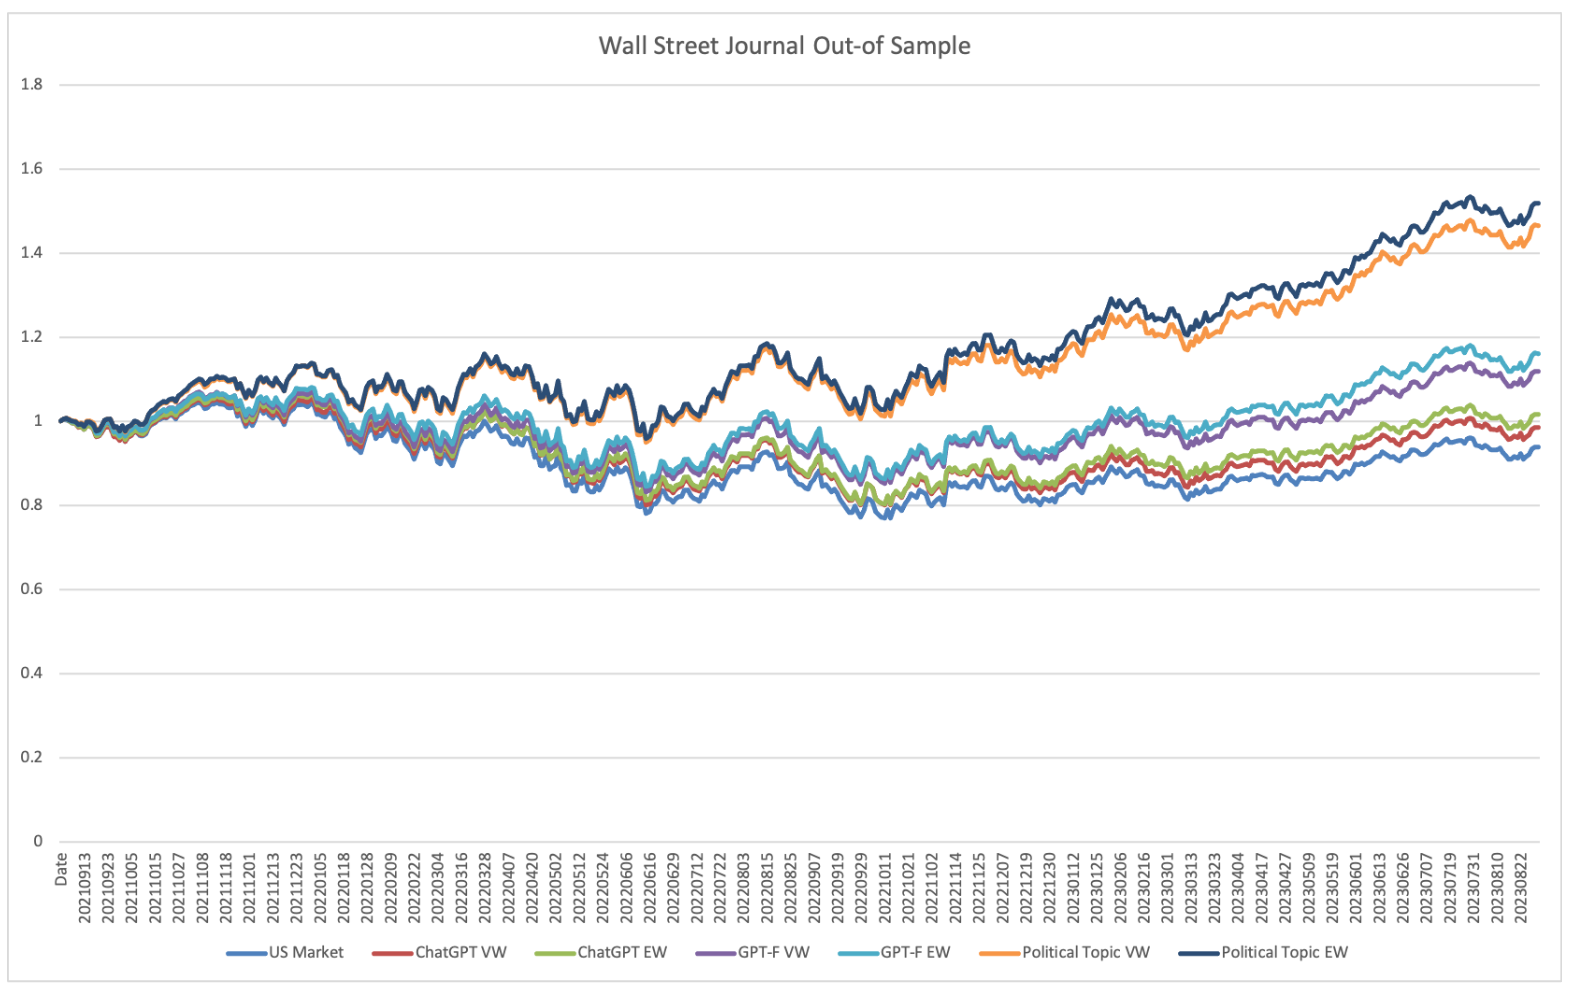
\includegraphics[width=0.9\textwidth]{fig/fig3.png}
    \caption*{Figure 3: Danh mục đầu tư ngoài mẫu từ Wall Street Journal}
    \label{fig:fig2}
\end{figure}
\textbf{Hình 3} minh họa lợi nhuận mua và giữ của danh mục ChatGPT so với danh mục thị trường ngoài mẫu.
\begin{itemize}
    \item Danh mục thị trường có lợi nhuận âm, ChatGPT (không tinh chỉnh) chỉ nhỉnh hơn chút.
    \item Sau tinh chỉnh, danh mục ChatGPT đạt lợi nhuận tích lũy \textbf{15-20\%} trong hai năm.
    \item Với chủ đề 3 (chính trị), lợi nhuận tăng đáng kể, tích lũy \textbf{40-50\%}.
\end{itemize}

\subsubsection*{Kết luận}
Kết quả cho thấy \textbf{tinh chỉnh ChatGPT cải thiện hiệu suất ngoài mẫu}, đặc biệt ở các chủ đề liên quan đến \textbf{chính trị, Covid-19, và chiến tranh Nga-Ukraine}. Điều này khẳng định tiềm năng của ChatGPT như công cụ hỗ trợ tư vấn tài chính hiệu quả.

\section{Testing ChatGPT sử dụng dữ liệu chính sách Trung Quốc}
Vì kết quả từ WSJ cho thấy ChatGPT hoạt động khá tốt trong bối cảnh tin tức chính sách, chúng tôi kiểm tra khả năng của ChatGPT trong việc đề xuất cổ phiếu dựa trên một nguồn khác, đó là tin tức chính sách ở Trung Quốc.
\\ Thị trường chứng khoán ở Trung Quốc bị chi phối mạnh mẽ bởi sự can thiệp của chính phủ (Capenter và Whitelaw 2017), do đó, dựa trên các kết quả từ Mỹ, nhóm tác giả đã giả định rằng kết quả sẽ áp dụng rất tốt trong thị trường chứng khoán Trung Quốc. Họ thu thập dữ liệu liên quan đến sự hỗ trợ chính sách ở cấp ngành từ cơ sở dữ liệu văn bản chính sách chính thức của Hội đồng Nhà nước, bao gồm các văn bản bản chính sách được công bố của Hội đồng Nhà nước, cũng như các văn bản từ nhiều bộ ngành và uỷ ban hoạt động dưới sự bảo trợ của Hội đồng Nhà nước Trung Quốc. 
\\Do Trung QUốc là một quốc gia do
trung ương quản lý, trao cho chính phủ quyền lực rộng rãi và khả năng điều chỉnh. Do đó, việc xây dựng và thực hiện các chính sách công nghiệp có ảnh hưởng đáng kể đến các thị trường tài chính. 
\begin{figure}[H]
    \centering
    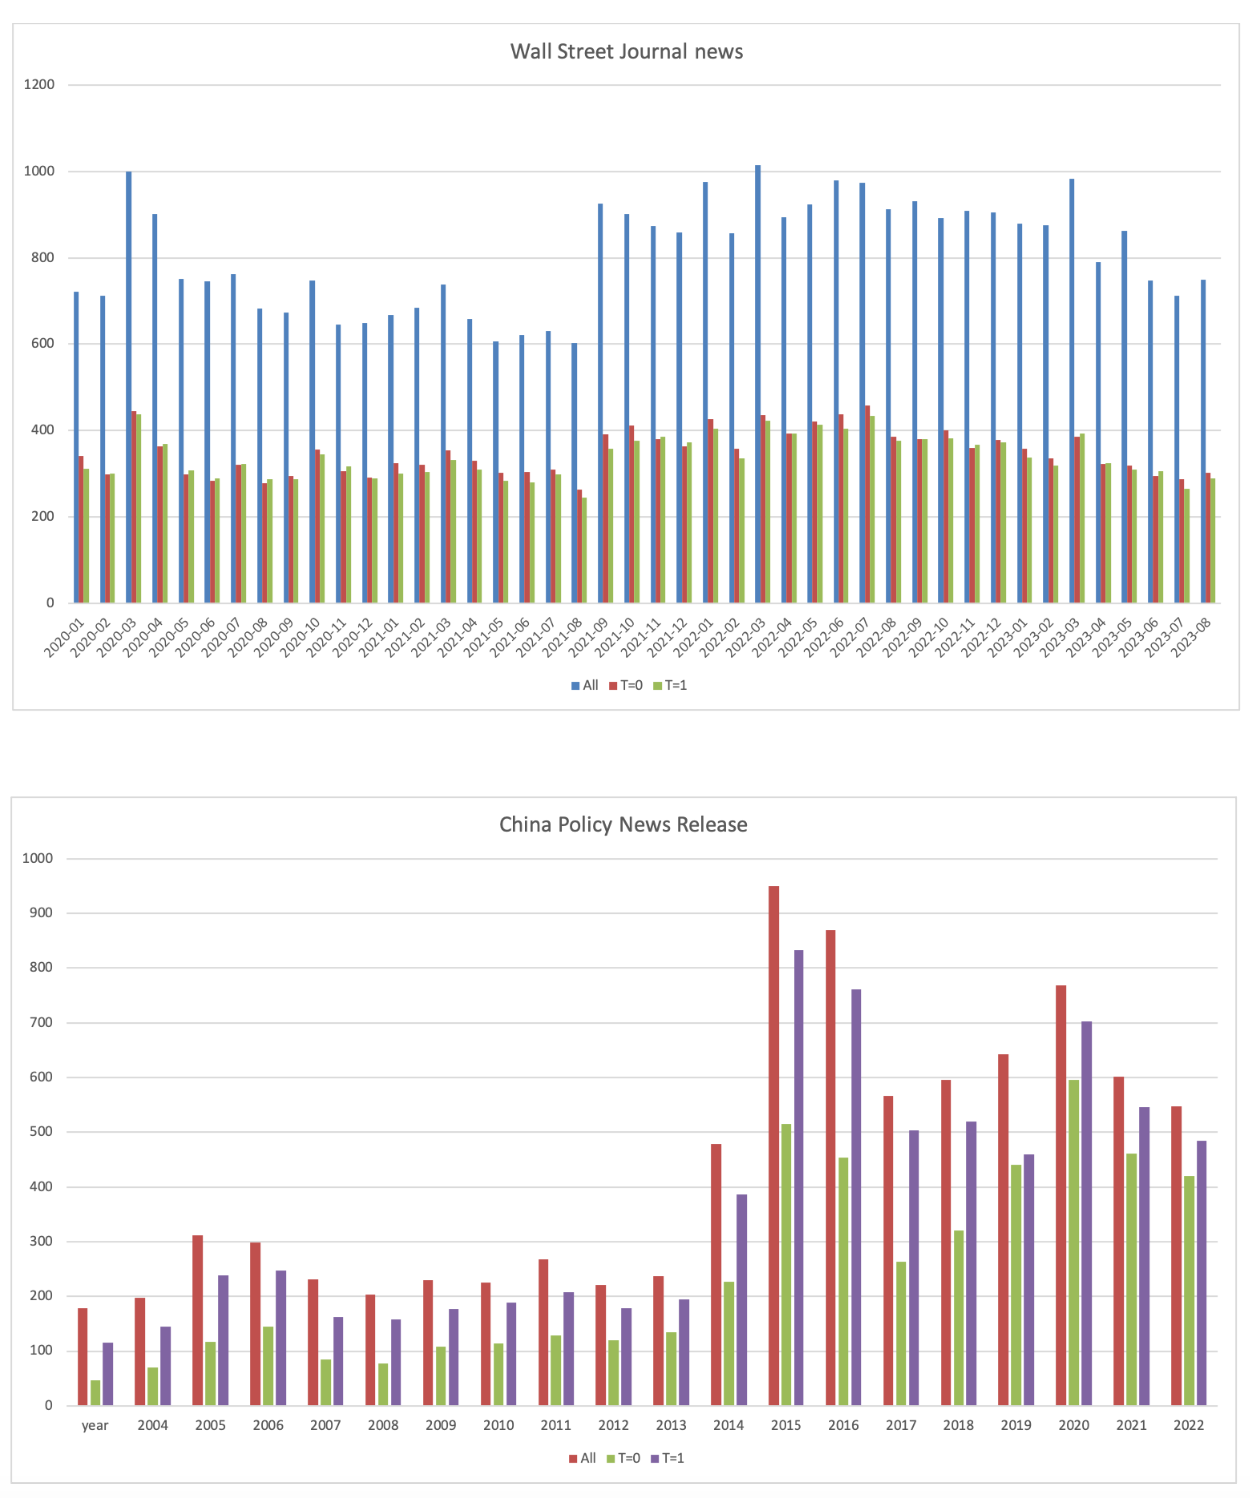
\includegraphics[width=0.8\textwidth]{fig/fig2.png}
    \label{fig:fig2}
\end{figure}
\textbf{Hình 2} cho thấy số lượng công bố tin tức chính sách theo năm trong giai đoạn mẫu của nhóm tác giả với tổng cộng hơn \textbf{8000 tin tức chính sách}. ChatGPT nhận thấy khoảng một nửa số công bố chính sách này là liên quan đến việc khuyến nghị cổ phiếu trong chuỗi thời gian. Kết quả này \textbf{không thay đổi nhiều} bởi tham số T mà nhóm tác giả đặt, tương tự như đối với Wall Street Journal.
\subsection{Bài kiểm tra lập luận dựa trên đánh giá của con người}

\subsubsection{Giới thiệu}
Sau khi tiến hành các kiểm tra lập luận với dữ liệu từ Wall Street Journal của Mỹ, nhóm nghiên cứu tiếp tục thực hiện kiểm tra khả năng lập luận của ChatGPT với dữ liệu \textbf{chính sách Trung Quốc}. Trung Quốc có hệ thống chính sách với đặc thù riêng, chịu sự điều tiết mạnh mẽ từ chính phủ, do đó nhóm giả định rằng kết quả lập luận của ChatGPT có thể phản ánh khả năng hiểu và phân tích nội dung chính sách trong bối cảnh đặc thù này.

\subsubsection{Phương pháp kiểm tra}
\begin{itemize}
    \item \textbf{Nguồn dữ liệu}: Văn bản chính sách được công bố bởi Hội đồng Nhà nước Trung Quốc và các cơ quan trực thuộc. Các tin tức chính sách được trích xuất từ cơ sở dữ liệu chính thức.
    \item \textbf{Quy trình đánh giá}: Tương tự với phần Wall Street Journal, nhóm nghiên cứu chọn ngẫu nhiên các tin tức chính sách từ Trung Quốc, yêu cầu ChatGPT đưa ra khuyến nghị đầu tư cổ phiếu hoặc ngành. Sau đó, các khuyến nghị này được đánh giá bởi nhóm đánh giá độc lập (bao gồm chuyên gia và người học trong lĩnh vực tài chính) theo ba tiêu chí:
    \begin{itemize}
        \item \textit{Tính liên quan (Relevance)} – nội dung có liên quan đến thị trường chứng khoán.
        \item \textit{Lý do hợp lý (Reasoning)} – lập luận có logic và phù hợp với thông tin từ dữ liệu chính sách.
        \item \textit{Cơ hội đầu tư (Investment Opportunity)} – tiềm năng sinh lời từ khuyến nghị.
    \end{itemize}
    \item \textbf{Phân loại kết quả}: Các khuyến nghị được phân loại thành ba nhóm: \textbf{Hợp lý (Logical)}, \textbf{Không rõ ràng (Unclear)}, và \textbf{Không liên quan (Unrelated)}.
\end{itemize}

\subsubsection{Kết quả đánh giá}
\begin{itemize}
    \item Tương tự với kết quả từ dữ liệu Wall Street Journal, ChatGPT thể hiện khả năng lập luận khá tốt trên dữ liệu chính sách Trung Quốc. Tỷ lệ khuyến nghị được đánh giá là \textbf{hợp lý} chiếm đa số, trong khi các khuyến nghị \textbf{không rõ ràng} và \textbf{không liên quan} có tỷ lệ thấp hơn đáng kể.
    \item Đặc biệt, việc thay đổi tham số nhiệt độ (\textbf{T=0} và \textbf{T=1}) không ảnh hưởng nhiều đến chất lượng lập luận của ChatGPT đối với dữ liệu chính sách Trung Quốc. Điều này cho thấy tính ổn định và khả năng phân tích chính sách của mô hình trong bối cảnh mới.
\end{itemize}

\subsubsection{Kết luận}
Kết quả kiểm tra lập luận từ dữ liệu chính sách Trung Quốc cho thấy ChatGPT có khả năng hiểu và phân tích nội dung chính sách trong bối cảnh đặc thù, đồng thời đưa ra các khuyến nghị đầu tư với tính hợp lý cao. Kết quả này cũng khẳng định rằng \textbf{mô hình ChatGPT có thể mở rộng áp dụng cho các thị trường khác nhau}, không chỉ ở Mỹ mà cả ở những thị trường có sự can thiệp của chính phủ mạnh mẽ như Trung Quốc.

\subsection{Thị trường chứng khoán Trung Quốc: Kiểm định trong mẫu (In sample test)}

Nghiên cứu tiến hành kiểm định trong mẫu để đánh giá hiệu quả của các danh mục đầu tư được ChatGPT đề xuất dựa trên các thông cáo chính sách của Quốc vụ viện Trung Quốc trong giai đoạn từ ngày 01/01/2014 đến ngày 30/08/2021. Đây là giai đoạn nằm trong tập huấn luyện của ChatGPT, cho phép kiểm tra khả năng khai thác thông tin từ văn bản chính sách mà mô hình có thể đã tiếp xúc trong quá trình tiền huấn luyện.

\subsubsection{Thiết kế thực nghiệm}
\begin{itemize}
    \item Dữ liệu văn bản: thông cáo chính sách chính thức từ Quốc vụ viện Trung Quốc.
    \item Các danh mục đầu tư được xây dựng dựa trên các khuyến nghị cổ phiếu của ChatGPT sau khi đọc từng thông cáo chính sách.
    \item Thời gian nắm giữ cổ phiếu trong danh mục gồm: 1 năm, 6 tháng, 3 tháng, 1 tháng, 1 tuần và 1 ngày.
    \item Hai phương pháp gán trọng số danh mục: \textbf{Equal-weighted (EW)} và \textbf{Value-weighted (VW)}.
    \item Đánh giá hiệu suất bằng hệ số alpha hàng ngày theo mô hình Fama-French 5 yếu tố mở rộng (bao gồm thêm yếu tố động lượng và đảo chiều).
\end{itemize}

\subsubsection{Kết quả thực nghiệm}
\begin{figure}[H]
    \centering
    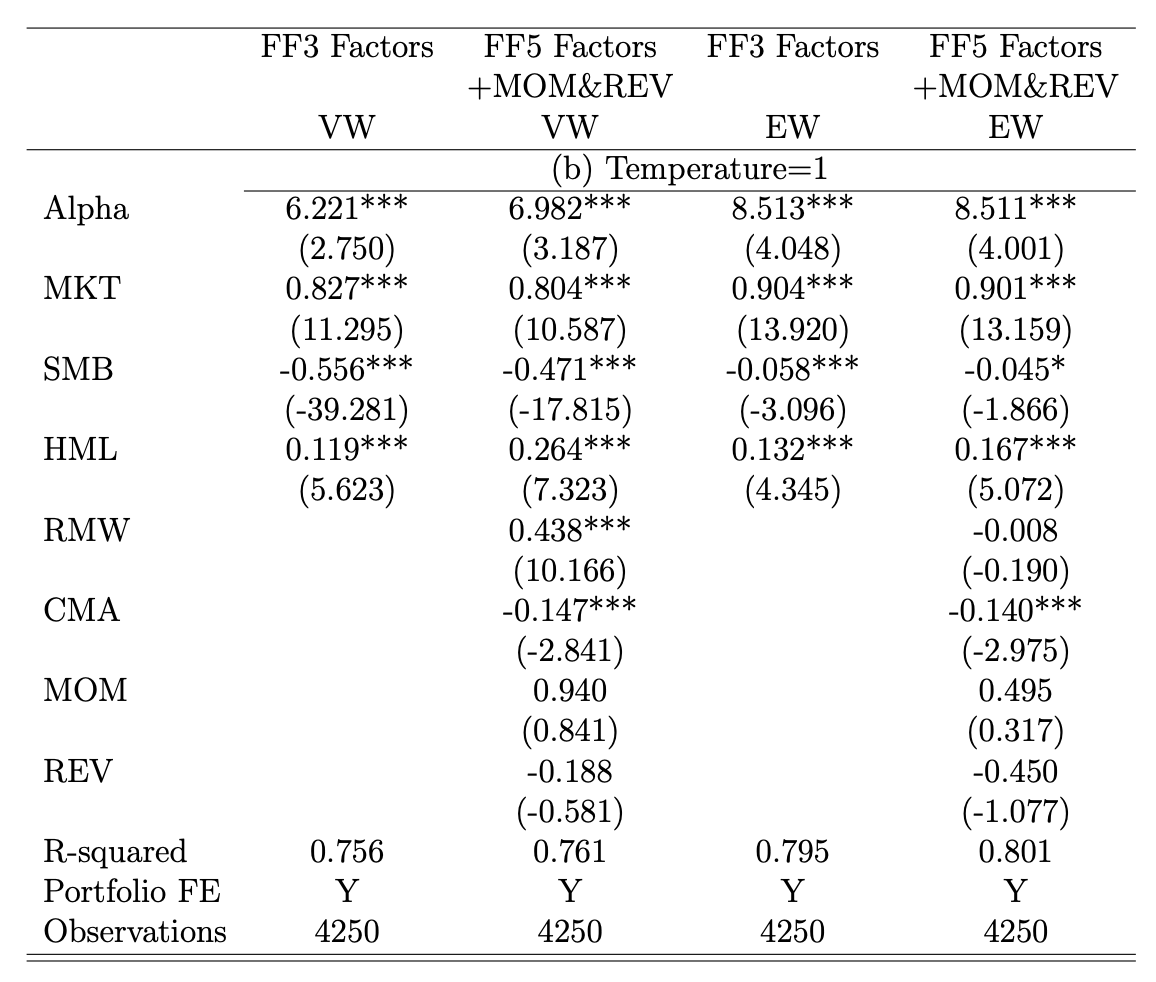
\includegraphics[width=0.8\textwidth]{table/tab9b.png}
    \caption*{Table 9: Kiểm định trong mẫu các khuyến nghị cổ phiếu dựa trên công bố chính sách của Quốc vụ viện Trung Quốc}
    \label{fig:fig2}
\end{figure}
\begin{itemize}
    \item Với \textbf{ChatGPT 3.5} và \textbf{T = 1} (nhiệt độ cao), danh mục nắm giữ trong vòng \textbf{1 tháng} cho kết quả vượt trội:
    \begin{itemize}
        \item Alpha hàng ngày (VW): \textbf{6.982 bps}, với $t$ = 3.187.
        \item Alpha hàng ngày (EW): \textbf{8.511 bps}, với $t$ = 4.001.
    \end{itemize}
    \item Các khoảng thời gian nắm giữ khác (1 năm, 6 tháng, 3 tháng, 1 tuần, 1 ngày) không cho thấy alpha có ý nghĩa thống kê hoặc nhất quán.
    \item Với \textbf{ChatGPT 4.0}, hiệu suất thấp hơn đáng kể:
    \begin{itemize}
        \item Với T = 1 và thời gian nắm giữ 1 tháng, alpha danh mục EW chỉ đạt \textbf{2.174 bps} (t = 1.019), không có ý nghĩa thống kê.
        \item Không có kết quả alpha đáng kể nào với VW trong toàn bộ các kỳ nắm giữ.
    \end{itemize}
\end{itemize}

\subsubsection{Kết luận}
Kết quả cho thấy ChatGPT 3.5 có khả năng tạo ra danh mục đầu tư vượt trội từ dữ liệu chính sách của chính phủ Trung Quốc, trong khi ChatGPT 4.0 lại không cho thấy hiệu quả tương tự trong giai đoạn in-sample. Điều này cho thấy:

\begin{itemize}
    \item Khả năng khai thác văn bản chính sách của ChatGPT phụ thuộc nhiều vào phiên bản mô hình và cấu hình tham số.
    \item Phiên bản 3.5 với phản hồi đa dạng (T = 1) khai thác tốt hơn các tín hiệu từ ngữ cảnh chính sách.
    \item Khả năng trích xuất thông tin từ văn bản tiếng Trung của ChatGPT được xác nhận là đủ mạnh để hỗ trợ xây dựng danh mục đầu tư có hiệu suất vượt trội.
\end{itemize}
\noindent
Kết quả kiểm định trong mẫu đối với chính sách Trung Quốc củng cố luận điểm rằng ChatGPT có thể được sử dụng hiệu quả như một công cụ phân tích văn bản tài chính, không chỉ ở thị trường Mỹ mà còn tại các thị trường chịu tác động chính sách mạnh như Trung Quốc.

\subsection{Thị trường cổ phiếu Trung Quốc: Kiểm định ngoài mẫu (Out-of-sample Test)}

\subsubsection{Giới thiệu và phương pháp}

Sau khi tiến hành kiểm định trong mẫu để đánh giá năng lực của ChatGPT trong việc đưa ra khuyến nghị đầu tư dựa trên các thông cáo chính sách của Quốc vụ viện Trung Quốc, nghiên cứu tiếp tục mở rộng sang giai đoạn kiểm định ngoài mẫu (out-of-sample). Giai đoạn này trải dài từ tháng 9 năm 2021 đến tháng 8 năm 2023 – tương ứng với khoảng thời gian mà dữ liệu chưa từng được mô hình tiếp cận trong quá trình huấn luyện, do đó là minh chứng quan trọng cho khả năng dự báo thực sự của ChatGPT trong bối cảnh thị trường thực tế.
\\Trong giai đoạn này, nhóm nghiên cứu tiếp tục sử dụng ChatGPT để đưa ra khuyến nghị cổ phiếu dựa trên các văn bản chính sách được công bố bởi chính phủ Trung Quốc. Cũng như trước đó, các danh mục được xây dựng theo hai phương pháp: giá trị bình quân đều (Equal-weighted – EW) và giá trị theo vốn hóa (Value-weighted – VW). Việc kiểm định hiệu suất danh mục được thực hiện bằng mô hình định giá tài sản Fama-French 5 yếu tố, bổ sung thêm hai yếu tố: động lượng (Momentum – MOM) và đảo chiều ngắn hạn (Reversal – REV). Hai mức nhiệt độ được xem xét: T=0 (không ngẫu nhiên) và T=1 (tăng tính sáng tạo).

\subsubsection{Thiết kế thực nghiệm}

Thiết kế kiểm định ngoài mẫu tương tự như giai đoạn in-sample, với các điểm chính như sau:

\begin{itemize}
    \item \textbf{Nguồn dữ liệu:} Các thông cáo chính sách từ Quốc vụ viện Trung Quốc được công bố trong giai đoạn 09/2021 – 08/2023.
    
    \item \textbf{Xử lý dữ liệu:} Mỗi văn bản chính sách được ChatGPT (phiên bản 3.5 và 4.0) phân tích và phản hồi bằng danh sách 5 cổ phiếu được đề xuất, tương ứng với nội dung của văn bản.
    
    \item \textbf{Thời gian nắm giữ danh mục:} 1 tháng cố định cho mỗi cổ phiếu được chọn.
    
    \item \textbf{Phương pháp gán trọng số:}
    \begin{itemize}
        \item \textbf{Equal-weighted (EW)}: Mỗi cổ phiếu trong danh mục có trọng số bằng nhau.
        \item \textbf{Value-weighted (VW)}: Trọng số theo vốn hóa thị trường.
    \end{itemize}
    
    \item \textbf{Phương pháp đánh giá hiệu suất:}  
    Hồi quy time-series alpha theo mô hình Fama-French 5 yếu tố mở rộng (FF5 + MOM + REV), trong đó:
    \begin{itemize}
        \item MOM: yếu tố đà tăng;
        \item REV: yếu tố đảo chiều ngắn hạn.
    \end{itemize}
    
    \item \textbf{Tham số nhiệt độ (temperature):}  
    So sánh hai mức:
    \begin{itemize}
        \item \textbf{T = 0}: phản hồi ổn định;
        \item \textbf{T = 1}: phản hồi sáng tạo và đa dạng hơn.
    \end{itemize}
    
    \item \textbf{Chủ đề chính sách:} Các văn bản được phân loại thành 10 chủ đề nội dung sử dụng mô hình phân loại chủ đề (LDA).
\end{itemize}

\subsubsection{Kết quả thực nghiệm}

Kết quả kiểm định được trình bày trong Bảng 10 của bài báo và cho thấy:
\begin{figure}[H]
    \centering
    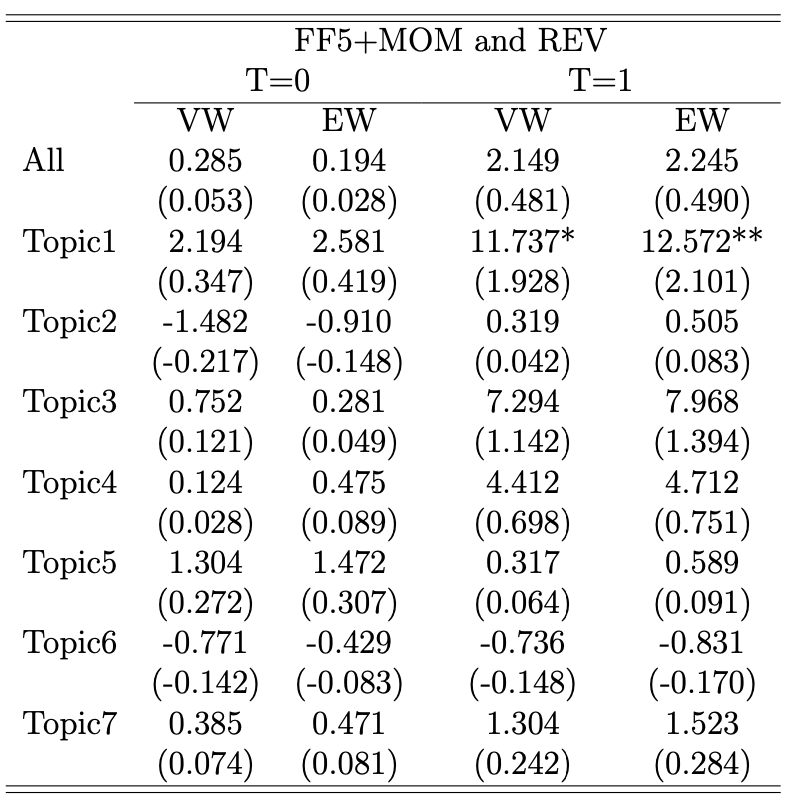
\includegraphics[width=0.7\textwidth]{table/tab10.png}
    \caption*{Table 10: Kiểm định ngoài mẫu các khuyến nghị cổ phiếu dựa trên công bố chính sách của Quốc vụ viện Trung Quốc}
    \label{fig:fig2}
\end{figure}
\begin{itemize}
    \item \textbf{Toàn bộ dữ liệu:} Khi sử dụng ChatGPT 3.5 với \textbf{T = 1}, alpha hàng ngày đạt:
    \begin{itemize}
        \item \textbf{2.245 bps} (Equal-weighted), 
        \item \textbf{2.149 bps} (Value-weighted),
    \end{itemize}
    tuy nhiên không có ý nghĩa thống kê ở mức 10\%.

    \item \textbf{Chủ đề 1 – Xây dựng và đầu tư công:}  
    Đây là chủ đề có hiệu suất vượt trội nhất trong kiểm định out-of-sample. Khi T = 1:
    \begin{itemize}
        \item Alpha hàng ngày (VW): \textbf{8.737 bps} ($t$ = 1.82, $p < 0.1$),
        \item Alpha hàng ngày (EW): \textbf{9.572 bps} ($t$ = 2.33, $p < 0.05$).
    \end{itemize}
    
    \item \textbf{Các chủ đề còn lại:}  
    Một số chủ đề khác có alpha dương nhưng thiếu ý nghĩa thống kê hoặc không nhất quán giữa EW và VW. Một số thậm chí cho alpha âm, cho thấy hiệu suất không ổn định.

    \item \textbf{So sánh phiên bản:} ChatGPT 3.5 tiếp tục thể hiện kết quả tốt hơn ChatGPT 4.0 trong hầu hết các cấu hình thử nghiệm.
\end{itemize}
\subsubsection{Kết luận}
Kiểm định ngoài mẫu trên thị trường cổ phiếu Trung Quốc xác nhận rằng ChatGPT, đặc biệt phiên bản 3.5 với nhiệt độ cao, có khả năng tạo ra các danh mục đầu tư sinh lời từ phân tích văn bản chính sách – nhưng hiệu suất chủ yếu phụ thuộc vào nội dung chủ đề. Đặc biệt, ChatGPT cho thấy năng lực suy luận mạnh mẽ khi xử lý thông tin liên quan đến đầu tư công, xây dựng hạ tầng và chính sách kinh tế vĩ mô.
\noindent
\\Kết quả này củng cố tiềm năng ứng dụng ChatGPT trong đầu tư tại các thị trường chịu tác động cao từ chính sách, như Trung Quốc, đồng thời nhấn mạnh vai trò của phân loại chủ đề và kiểm soát tham số trong quá trình ứng dụng thực tế.
\subsection{Thị trường chứng khoán Trung Quốc: Kết quả sau tinh chỉnh mô hình (Fine-Tuning)}

\subsubsection{Giới thiệu}
Sau khi đánh giá hiệu suất của các khuyến nghị đầu tư do ChatGPT tạo ra từ tin tức chính sách Trung Quốc, nhóm tác giả tiếp tục thực hiện giai đoạn tinh chỉnh (fine-tuning) để kiểm tra xem việc cải thiện mô hình thông qua lọc lựa đầu ra có thể giúp nâng cao hiệu quả dự đoán trong giai đoạn kiểm định ngoài mẫu hay không. Phương pháp này không yêu cầu huấn luyện lại mô hình mà chỉ áp dụng điều chỉnh sau bước dự đoán đầu tiên.

\subsubsection{Phương pháp tinh chỉnh}
Cụ thể, sau khi ChatGPT đưa ra danh sách cổ phiếu đề xuất từ từng bài thông cáo chính sách, nhóm nghiên cứu chọn ra cổ phiếu \textbf{có hiệu suất thực tế cao nhất trong cùng ngành} (dựa trên mã ngành SIC) với cổ phiếu được đề xuất. Cách tiếp cận này nhằm duy trì tính hợp lý ngành nghề của khuyến nghị ban đầu, đồng thời tận dụng dữ liệu thị trường thực tế để tối ưu hóa kết quả đầu tư.

\subsubsection{Thiết kế thực nghiệm}
Các danh mục cổ phiếu được xây dựng dựa trên hai phương pháp phân bổ: tỷ trọng bằng nhau (equal-weighted - EW) và tỷ trọng theo vốn hóa (value-weighted - VW). Các chỉ số đánh giá chính bao gồm hệ số alpha từ mô hình Fama-French 5 yếu tố mở rộng (bao gồm cả yếu tố đà tăng MOM và đảo chiều REV). Giai đoạn kiểm định ngoài mẫu kéo dài từ tháng 9 năm 2021 đến tháng 2 năm 2024. Các thử nghiệm được thực hiện với hai mức \textit{temperature} (T=0 và T=1).

\subsubsection{Kết quả thực nghiệm}
Kết quả tổng thể khi áp dụng fine-tuning cho toàn bộ các chủ đề cho thấy:
\begin{figure}[H]
    \centering
    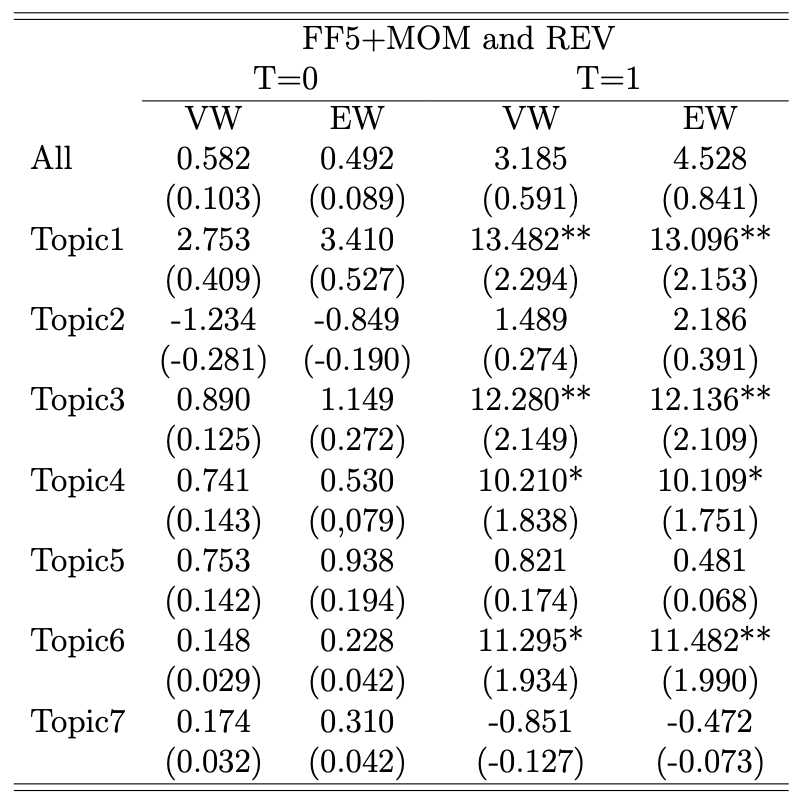
\includegraphics[width=0.5\textwidth]{table/tab11.png}
    \caption*{Table 11: Alpha của cổ phiếu được khuyến nghị dựa trên công bố chính sách của Quốc vụ viện Trung Quốc trong các kiểm định ngoài mẫu.}
    \label{fig:fig2}
\end{figure}
\begin{itemize}
    \item Với T=0: alpha của danh mục VW là 0.582 bps và EW là 0.492 bps – đều không có ý nghĩa thống kê.
    \item Với T=1: alpha tăng lên 3.185 bps (VW) và 4.528 bps (EW), tuy vẫn không có ý nghĩa thống kê, nhưng cho thấy xu hướng cải thiện hiệu suất đầu tư sau tinh chỉnh.
\end{itemize}

Xét riêng theo từng chủ đề, một số chủ đề thể hiện hiệu suất vượt trội đáng kể:

\begin{itemize}
    \item \textbf{Chủ đề 1 (đầu tư công, xây dựng)}: Alpha sau fine-tuning tăng mạnh với VW đạt 13.482 bps và EW đạt 13.096 bps, có ý nghĩa thống kê ở mức 1\%. Đây là nhóm chủ đề đem lại hiệu quả cao nhất sau tinh chỉnh.
    \item \textbf{Chủ đề 3 (địa chính trị)} và \textbf{Chủ đề 4 (COVID, ESG)}: Alpha đều đạt hơn 10 bps cho cả hai loại danh mục và có ý nghĩa thống kê ở mức 5\%.
    \item \textbf{Chủ đề 6}: Alpha đạt 11.295 bps (VW) và 11.482 bps (EW), có ý nghĩa lần lượt ở mức 10\% và 5\%.
    \item Các chủ đề còn lại (2, 5, 7) có alpha dương nhưng không có ý nghĩa thống kê.
\end{itemize}

\subsubsection{So sánh với phương pháp phân tích truyền thống}
\begin{figure}[H]
    \centering
    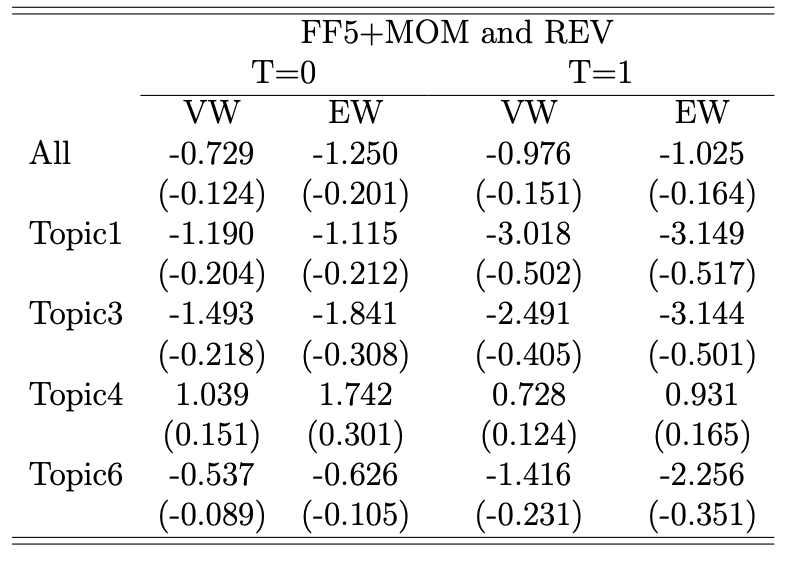
\includegraphics[width=0.6\textwidth]{table/tab12.png}
    \caption*{Table 12: Đối chiếu công bố chính sách của Quốc vụ viện Trung Quốc với phân tích văn bản truyền thống.}
    \label{fig:fig2}
\end{figure}
Để đối chứng, nhóm tác giả sử dụng phương pháp phân tích văn bản truyền thống – cụ thể là đo độ tương đồng cosine giữa văn bản tin tức và các báo cáo tài chính hoặc earning calls của doanh nghiệp. Kết quả từ phương pháp này không tạo ra bất kỳ danh mục nào có alpha dương có ý nghĩa thống kê, cho thấy sự vượt trội của ChatGPT sau khi được tinh chỉnh.

\subsubsection{Tổng kết}
Kết quả cho thấy quá trình fine-tuning đơn giản, không cần can thiệp vào nội tại mô hình, đã giúp cải thiện đáng kể hiệu suất của các danh mục đầu tư do ChatGPT tạo ra, đặc biệt trong bối cảnh tin tức chính sách. Phương pháp này cho thấy tiềm năng ứng dụng ChatGPT như một khung suy luận (reasoning framework) kết hợp với tín hiệu định lượng để đưa ra quyết định đầu tư có hiệu quả trong thực tế.

\section{Kiểm tra tính ổn định}

\subsection{Thiết kế kiểm tra}

Để kiểm tra độ ổn định và độ chắc chắn trong khả năng dự báo của ChatGPT, nhóm tác giả đã thực hiện một thử nghiệm kiểm chứng bằng cách giới hạn thông tin đầu vào của mô hình chỉ còn phần \textbf{tiêu đề} của các bản tin chính sách. Mục đích là kiểm tra xem liệu ChatGPT vẫn có thể tạo ra khuyến nghị đầu tư có ý nghĩa chỉ với thông tin hạn chế như vậy, từ đó xác định mức độ giá trị gia tăng thực sự đến từ khả năng hiểu toàn văn bản của mô hình.

\subsection{Kết quả kiểm tra}

Kết quả cho thấy rằng khi chỉ sử dụng phần tiêu đề, \textbf{không có danh mục đầu tư nào tạo ra alpha có ý nghĩa thống kê} theo mô hình ba yếu tố hoặc năm yếu tố, dù là trên dữ liệu từ Wall Street Journal (Mỹ) hay thông cáo chính sách Trung Quốc. Điều này cho thấy rằng ChatGPT \textbf{phụ thuộc đáng kể vào thông tin chi tiết trong nội dung đầy đủ của văn bản} để đưa ra các dự đoán chính xác và hiệu quả đầu tư cao.
\noindent
Ngoài ra, khi so sánh với các phương pháp phân tích văn bản truyền thống như đo độ tương đồng cosine giữa bản tin và báo cáo tài chính hoặc cuộc gọi thu nhập của các công ty, các phương pháp này \textbf{không tạo ra danh mục có alpha dương đáng kể}, cho thấy sự vượt trội của ChatGPT trong khả năng trích xuất và suy luận từ thông tin phi cấu trúc.

\section{Kết luận}

Trong nghiên cứu này, nhóm tác giả đã kiểm tra liệu một mô hình ngôn ngữ lớn như ChatGPT có thể hỗ trợ nhà đầu tư ra quyết định dựa trên khả năng suy luận ngôn ngữ từ các dữ liệu văn bản phức tạp hay không. Thay vì dựa vào mô hình học máy có giám sát truyền thống, ChatGPT sử dụng khả năng học từ ngữ cảnh và suy luận để đưa ra khuyến nghị đầu tư mà không cần cấu trúc dữ liệu cố định.

\textbf{Kết quả chính} cho thấy rằng ChatGPT:
\begin{itemize}
    \item Có khả năng hiểu và liên hệ thông tin từ bản tin chính sách với cổ phiếu cụ thể một cách hiệu quả hơn các phương pháp truyền thống.
    \item Tạo ra danh mục đầu tư có alpha dương và có ý nghĩa thống kê, đặc biệt là với các chủ đề như đầu tư công, xây dựng, chính trị, ESG.
    \item Hoạt động tốt ngay cả khi xử lý ngôn ngữ không phải tiếng Anh, như trong trường hợp phân tích chính sách Trung Quốc.
    \item Cho thấy hiệu suất được cải thiện rõ rệt khi thực hiện tinh chỉnh (fine-tuning) đơn giản dựa trên mã ngành (SIC), cho thấy tiềm năng kết hợp giữa mô hình ngôn ngữ tổng quát và kiến thức chuyên ngành.
\end{itemize}
\noindent
Nghiên cứu khẳng định tiềm năng ứng dụng của ChatGPT như một công cụ hỗ trợ đầu tư (robo-advisor) thông minh, giúp nhà đầu tư khai thác tốt hơn các nguồn dữ liệu văn bản phi cấu trúc như tin tức, chính sách và báo cáo. ChatGPT mở ra một hướng đi mới trong việc áp dụng Generative AI vào lĩnh vực tài chính định lượng, đặc biệt trong môi trường ngày càng bị ảnh hưởng bởi thông tin thời sự và yếu tố phi định lượng.

\renewcommand{\refname}{Tài liệu tham khảo}
\begin{thebibliography}{99}

\bibitem{alsabah2021}
Alsabah, H., Capponi, A., Ruiz Lacedelli, O., \& Stern, M. (2021). Robo-advising: Learning investors risk preferences via portfolio choices. \textit{Journal of Financial Econometrics}, 19, 369-392.

\bibitem{capponi2022}
Capponi, A., Olafsson, S., \& Zariphopoulou, T. (2022). Personalized robo-advising: Enhancing investment through client interaction. \textit{Management Science}, 68, 2485-2512.

\bibitem{carpenter2017}
Carpenter, J. N., \& Whitelaw, R. F. (2017). The development of China's stock market and stakes for the global economy. \textit{Annual Review of Financial Economics}, 9, 233-257.

\bibitem{chen2023}
Chen, Y., Kelly, B., \& Xiu, D. (2023). Expected returns and foundation models of language. \textit{SSRN Working Paper}.

\bibitem{cong2022}
Cong, L. W., Feng, G., He, J., \& He, X. (2022). Growing the efficient frontier on panel trees. \textit{Journal of Financial Economics}.

\bibitem{cong2024a}
Cong, L. W., Feng, G., He, J., \& Wang, Y. (2024a). Mosaics of predictability. \textit{NBER Working Paper}.

\bibitem{cong2024b}
Cong, L. W., Liang, T., Zhang, X., \& Zhu, W. (2024b). Textual factors: A scalable, interpretable, and data-driven approach to analyzing unstructured information. \textit{NBER Working Paper}.

\bibitem{cong2019}
Cong, L. W., Tang, K., Wang, J., \& Zhang, Y. (2019). AlphaPortfolio: Direct construction through deep reinforcement learning and interpretable AI. \textit{SSRN Working Paper}.

\bibitem{dacunto2019}
DAcunto, F., Prabhala, N., \& Rossi, A. G. (2019). The promises and pitfalls of robo-advising. \textit{The Review of Financial Studies}, 32, 1983-2020.

\bibitem{eisfeldt2023}
Eisfeldt, A., Schubert, G., Taska, B., \& Zhang, M. (2023). Generative AI and firm values. \textit{SSRN Working Paper}.

\bibitem{fama2016}
Fama, E. F., \& French, K. R. (2016). Dissecting anomalies with a five-factor model. \textit{The Review of Financial Studies}, 29, 69-103.

\bibitem{gentzkow2019}
Gentzkow, M., Kelly, B., \& Taddy, M. (2019). Text as data. \textit{Journal of Economic Literature}, 57, 535-574.

\bibitem{giglio2021}
Giglio, S., Liao, Y., \& Xiu, D. (2021). Thousands of alpha tests. \textit{The Review of Financial Studies}, 34, 3456-3496.

\bibitem{gu2020}
Gu, S., Kelly, B., \& Xiu, D. (2020). Empirical asset pricing via machine learning. \textit{The Review of Financial Studies}, 33, 2223-2273.

\bibitem{jha2023}
Jha, M., Qian, J., Weber, M., \& Yang, B. (2023). ChatGPT and corporate policies. \textit{SSRN Working Paper}.

\bibitem{jiang2022}
Jiang, J., Kelly, B. T., \& Xiu, D. (2022). (Re-)imag(in)ing price trends. \textit{Journal of Finance}.

\bibitem{kelly2023}
Kelly, B., \& Xiu, D. (2023). Financial machine learning. \textit{SSRN Working Paper}.

\bibitem{kelly2022}
Kelly, B. T., Malamud, S., \& Zhou, K. (2022). The virtue of complexity in return prediction. \textit{SSRN Working Paper}.

\bibitem{loughran2011}
Loughran, T., \& McDonald, B. (2011). When is a liability not a liability? Textual analysis, dictionaries, and 10-Ks. \textit{The Journal of Finance}, 66, 35-65.

\bibitem{sheng2024}
Sheng, J., Sun, Z., Yang, B., \& Zhang, A. L. (2024). Generative AI and asset management. \textit{SSRN Working Paper}.

\bibitem{ssrn2023}
Zhang, Z., Chen, J., \& Shi, Y. (2023). ChatGPT's Reasoning Ability and Potential in Stock Selection Based on News. \textit{SSRN Electronic Journal}. DOI: 10.2139/ssrn.4519182.

\bibitem{fama1993}
Fama, E. F., \& French, K. R. (1993). Common risk factors in the returns on stocks and bonds. \textit{Journal of Financial Economics}, 33(1), 3-56.

\bibitem{fama2015}
Fama, E. F., \& French, K. R. (2015). A five-factor asset pricing model. \textit{Journal of Financial Economics}, 116(1), 1-22.

\bibitem{jegadeesh1993}
Jegadeesh, N., \& Titman, S. (1993). Returns to buying winners and selling losers: Implications for stock market efficiency. \textit{The Journal of Finance}, 48(1), 65-91.

\end{thebibliography}
\end{document}